\section{Drone Setup}
In this section, things tends to be my bespoke and my instructions will start to become more arbitary and generalised as the configuration differs for each drone. To appericate the process, this section provides a working list of a functional commmunication way of working. 

\subsection{Hardware Required}
You will need an ESP8266 Wifi Module, a Pixhawk6C, a Radio Controller, IR Markers, and of course, your drone. You need to setup your drone so that you can host a wifi network for your ground control station to connect to. I used an ESP8266 wifi chip for this, althought you are more than welcome (encouraged even) to explore using host wifi features from raspberry pi, which is known to be more stable than the ESP8266. \cite{grace}\\

The flight controller I am using is the Pixhawk 6C, do note that not all Pixhawk works the same when setting up the serial port, so this is just an arbitary example given that works. 
\begin{figure}[H]
    \centering
    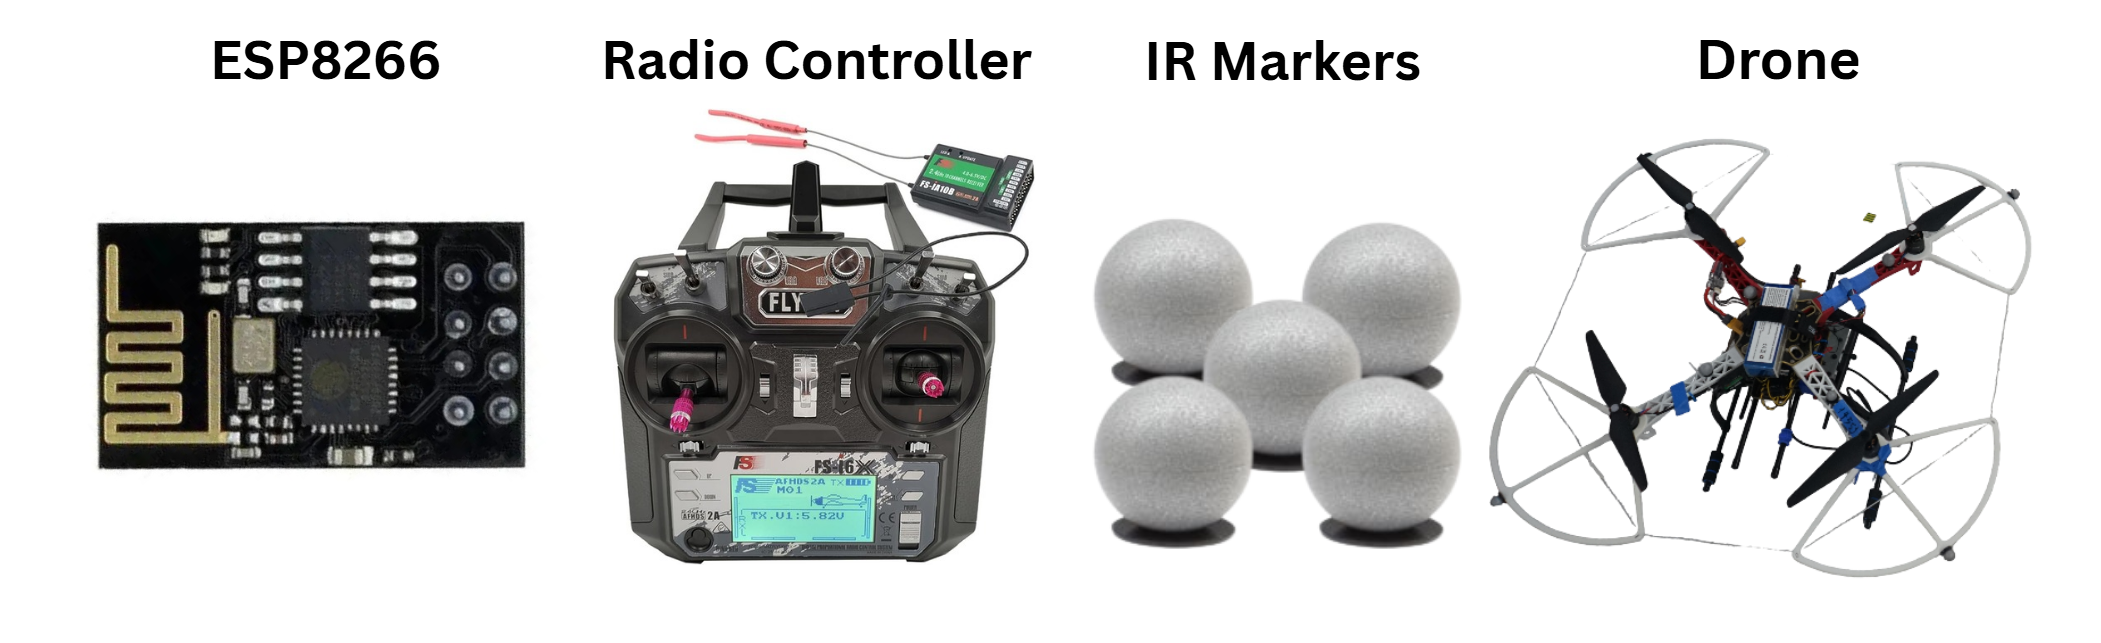
\includegraphics[width=1\linewidth]{Images/Hardware Requirements Drone.png}
    \caption{Hardware Required.}
    \label{fig:placeholder2}
\end{figure}

\subsection{ESP8266 to PixHawk6C}
\label{sec:hostport}
The ESP8266 to Pixhawk pinout is as follows:
\begin{figure}[H]
    \centering
    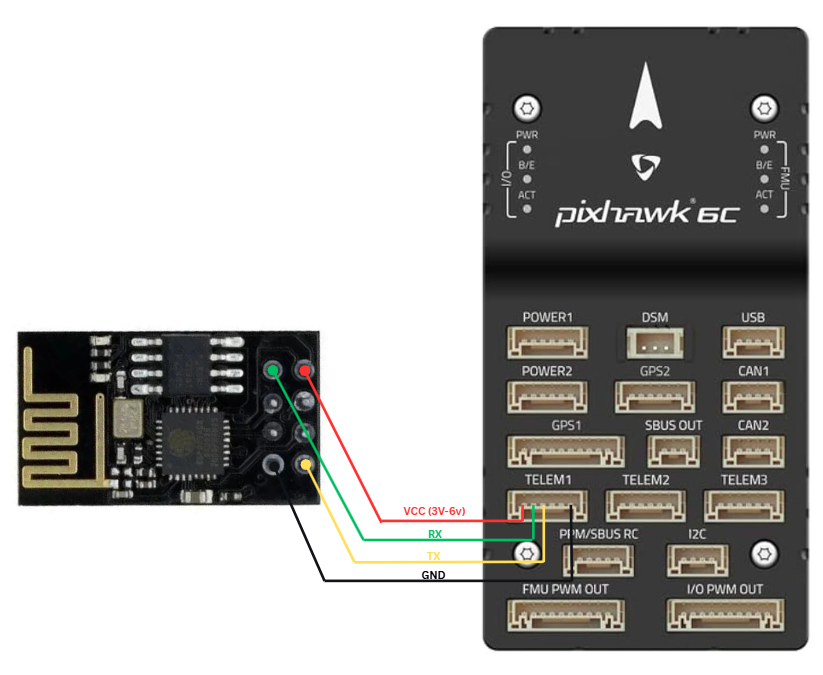
\includegraphics[width=0.6\linewidth]{Images/PinoutGood.png}
    \caption{Pinout from Pixhawk 6c to ESP8266.}
    \label{fig:placeholder2}
\end{figure}

Power up the Pixhawk (Remove the propellers). If the ESP8266 is being used for the 1st time, please see \cite{engineeringprojects_esp8266} for setting up wifi name and password. \textbf{(If you are using the drone after the 2025/2026 cohort, it is named as Inspector/Surveyour with password being inspector/surveyor correspondingly)}. Connect your GCS to the wifi as shown in figure \ref{fig:wifi1}
\begin{figure}[H]
    \centering
    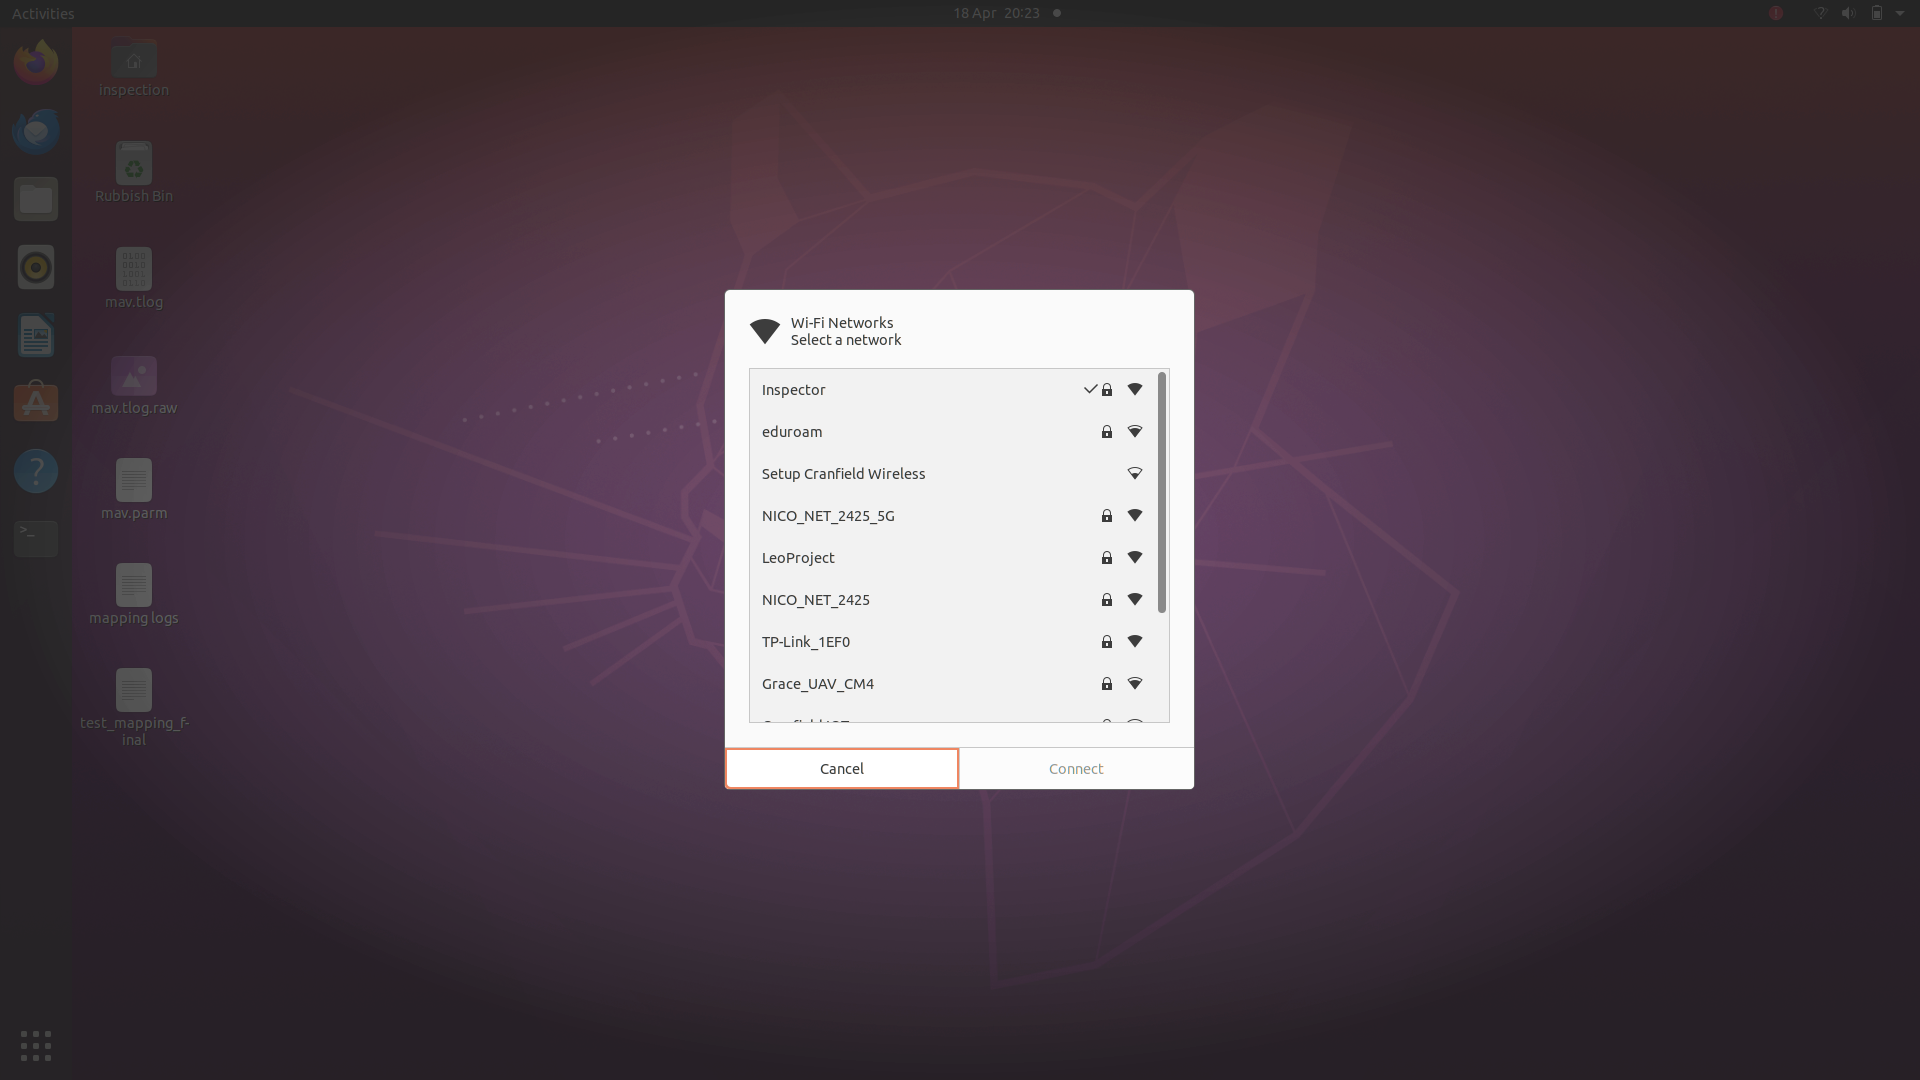
\includegraphics[width=1\linewidth]{Images/Wifi1.png}
    \caption{Pinout from Pixhawk 6c to ESP8266.}
    \label{fig:wifi1}
\end{figure}
Open your wifi setting as shown in \ref{fig:wifi3}: 
\begin{figure}[H]
    \centering
    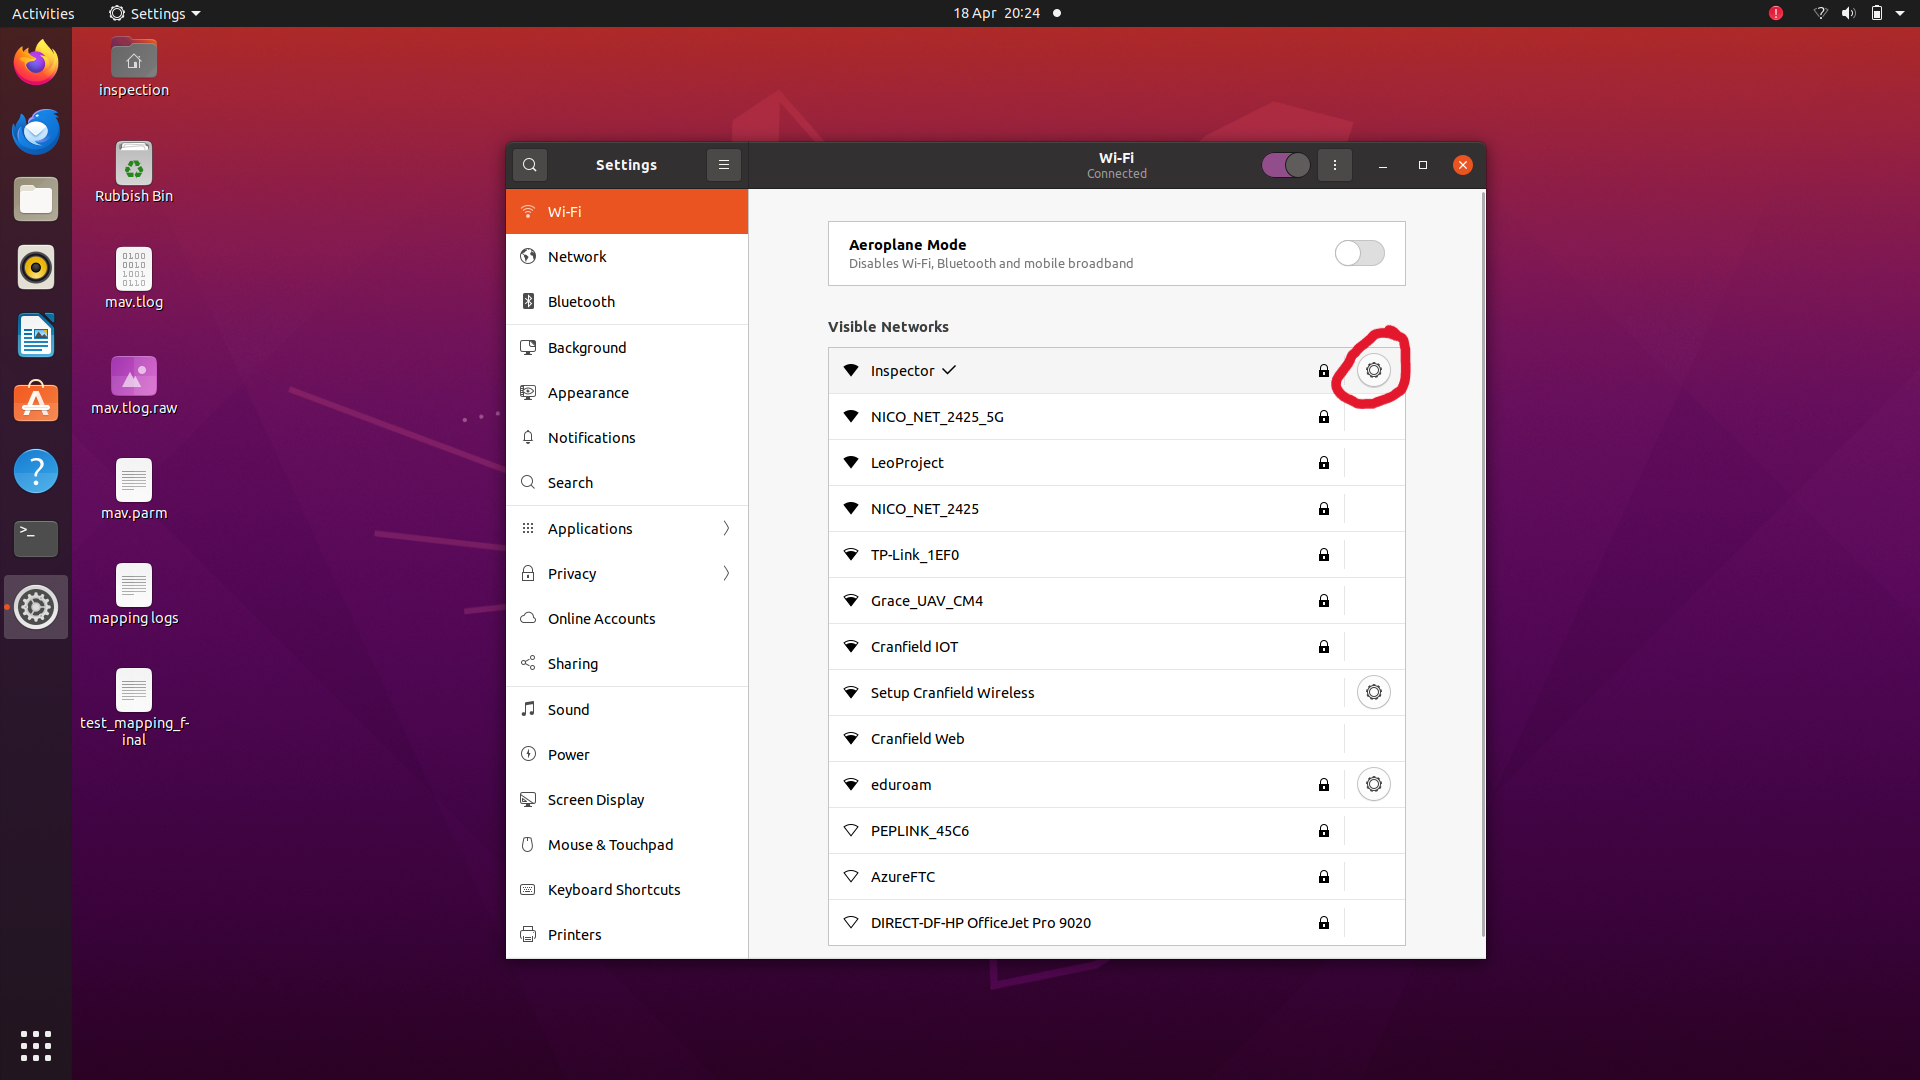
\includegraphics[width=1\linewidth]{Images/Wifi3.png}
    \caption{Pinout from Pixhawk 6c to ESP8266.}
    \label{fig:wifi3}
\end{figure}
Note down the WiFi's Default Route as seen in figure \ref{fig:wifi4}: 
\begin{figure}[H]
    \centering
    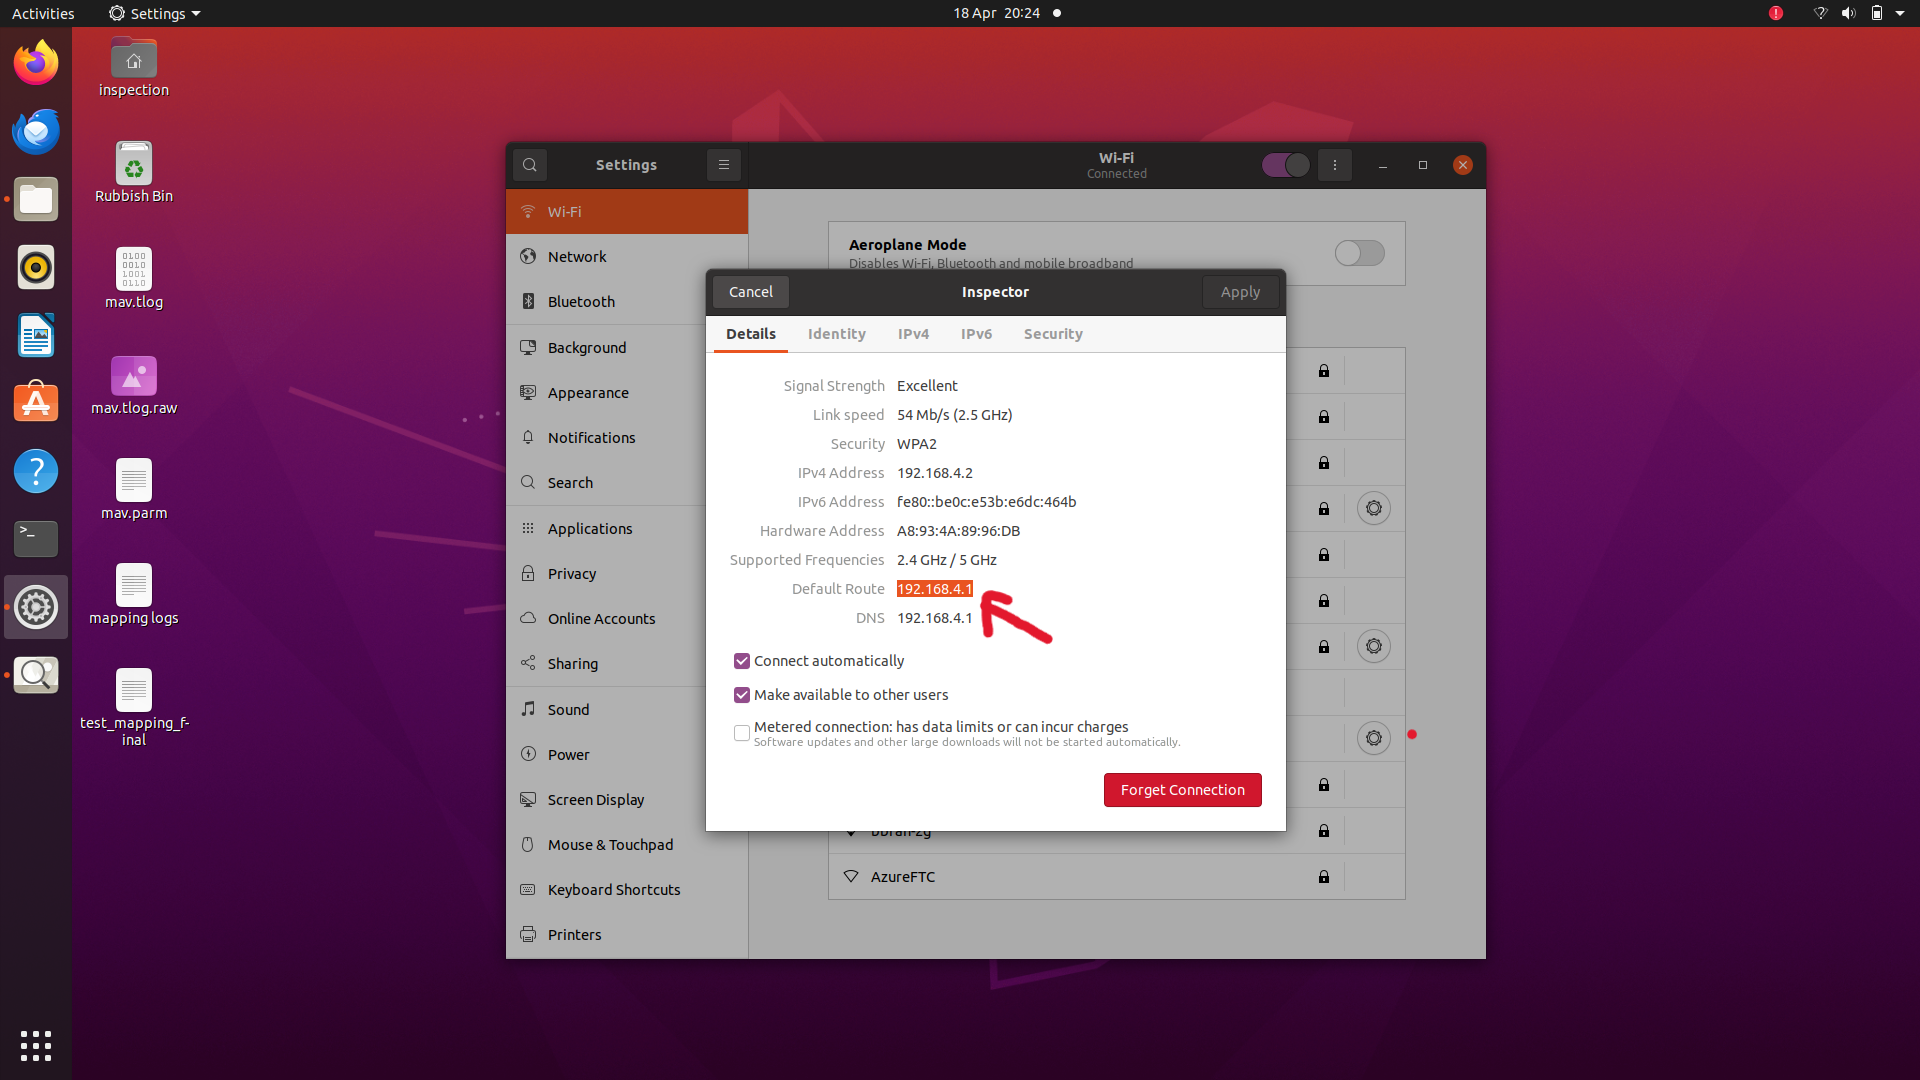
\includegraphics[width=1\linewidth]{Images/Wifi4.png}
    \caption{Pinout from Pixhawk 6c to ESP8266.}
    \label{fig:wifi4}
\end{figure}

Enter the wifi's default route into a browser, you should see a page as shown in figure \ref{fig:wifi6} below:

\begin{figure}[H]
    \centering
    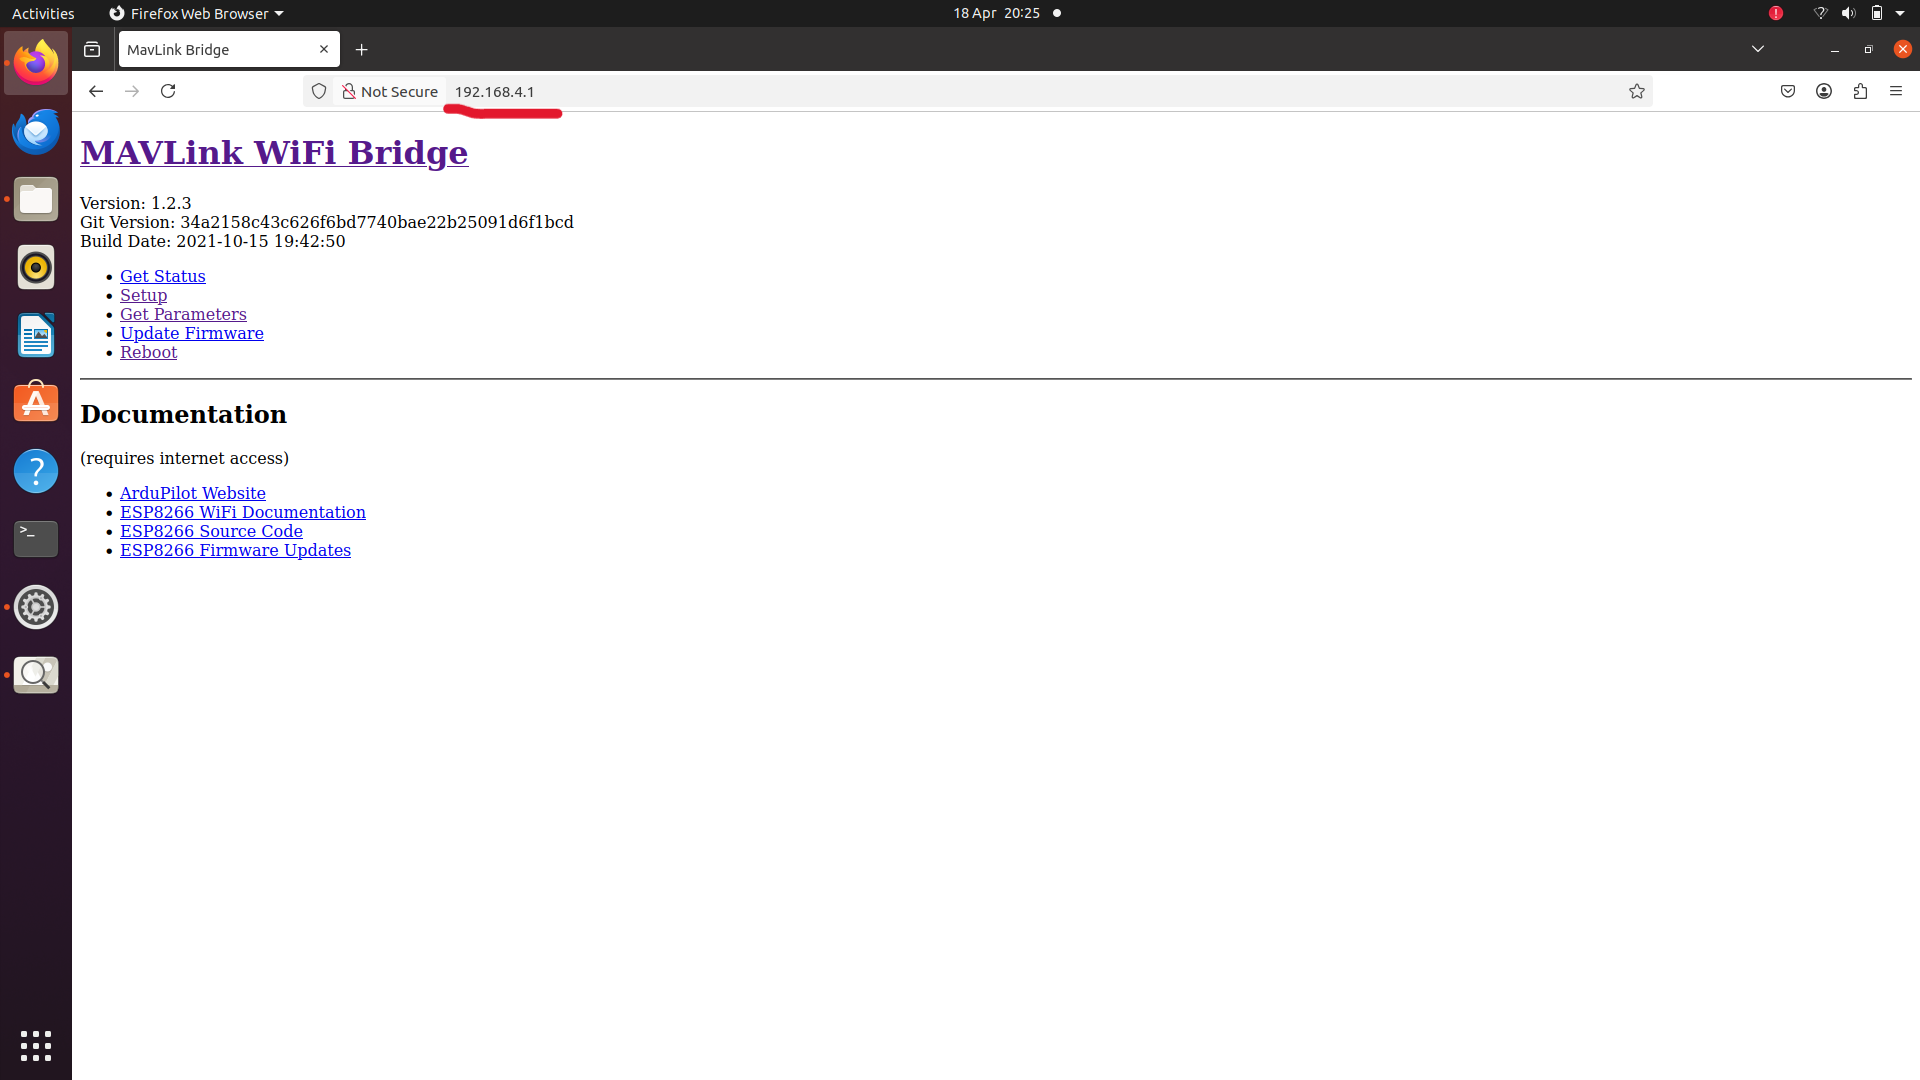
\includegraphics[width=1\linewidth]{Images/Wifi6.png}
    \caption{Pinout from Pixhawk 6c to ESP8266.}
    \label{fig:wifi6}
\end{figure}
Press \textit{Setup}, change your wifi SSID and password as you wish. Noting your host port's digit for later, as shown in figure \ref{fig:wifi7} 
\begin{figure}[H]
    \centering
    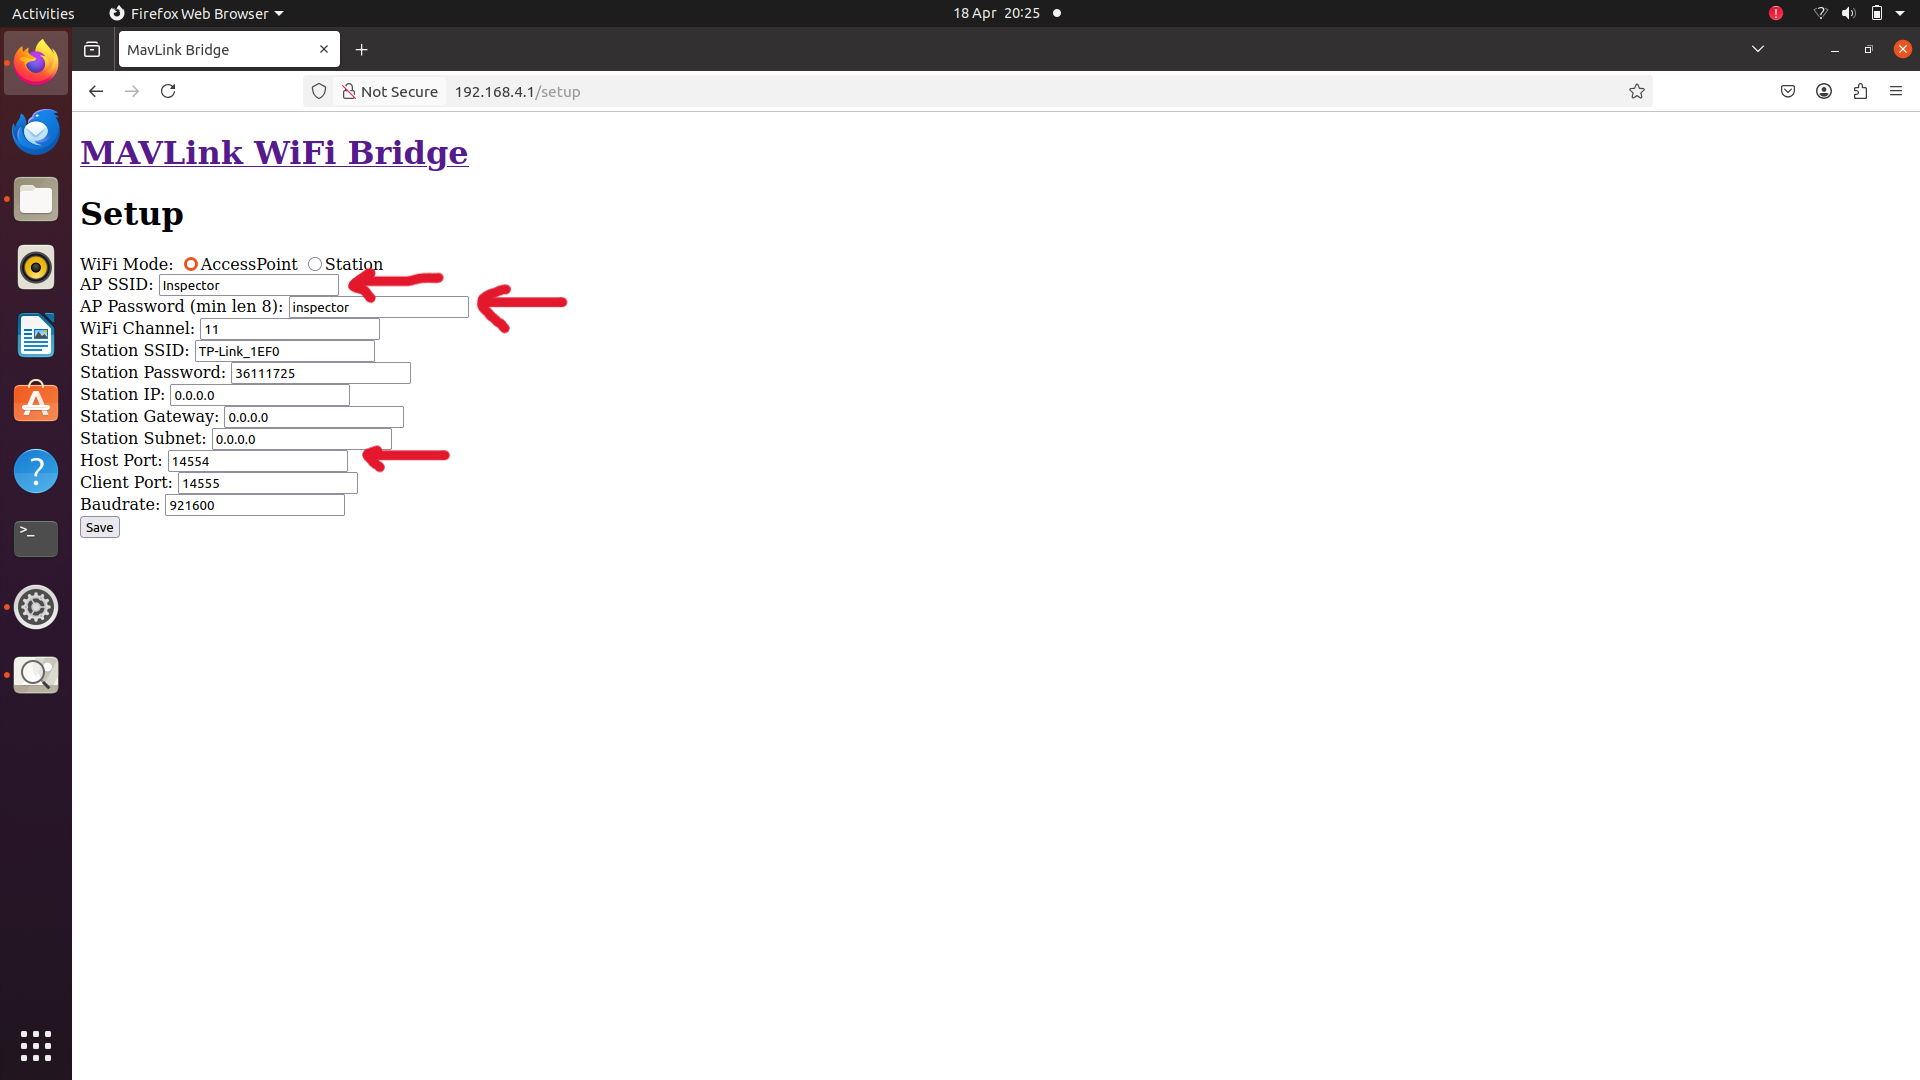
\includegraphics[width=1\linewidth]{Images/Wifi7.png}
    \caption{Pinout from Pixhawk 6c to ESP8266.}
    \label{fig:wifi7}
\end{figure}
Return to the home page, and press \textit{Reboot}, as shown in \ref{fig:wifi9}: 
\begin{figure}[H]
    \centering
    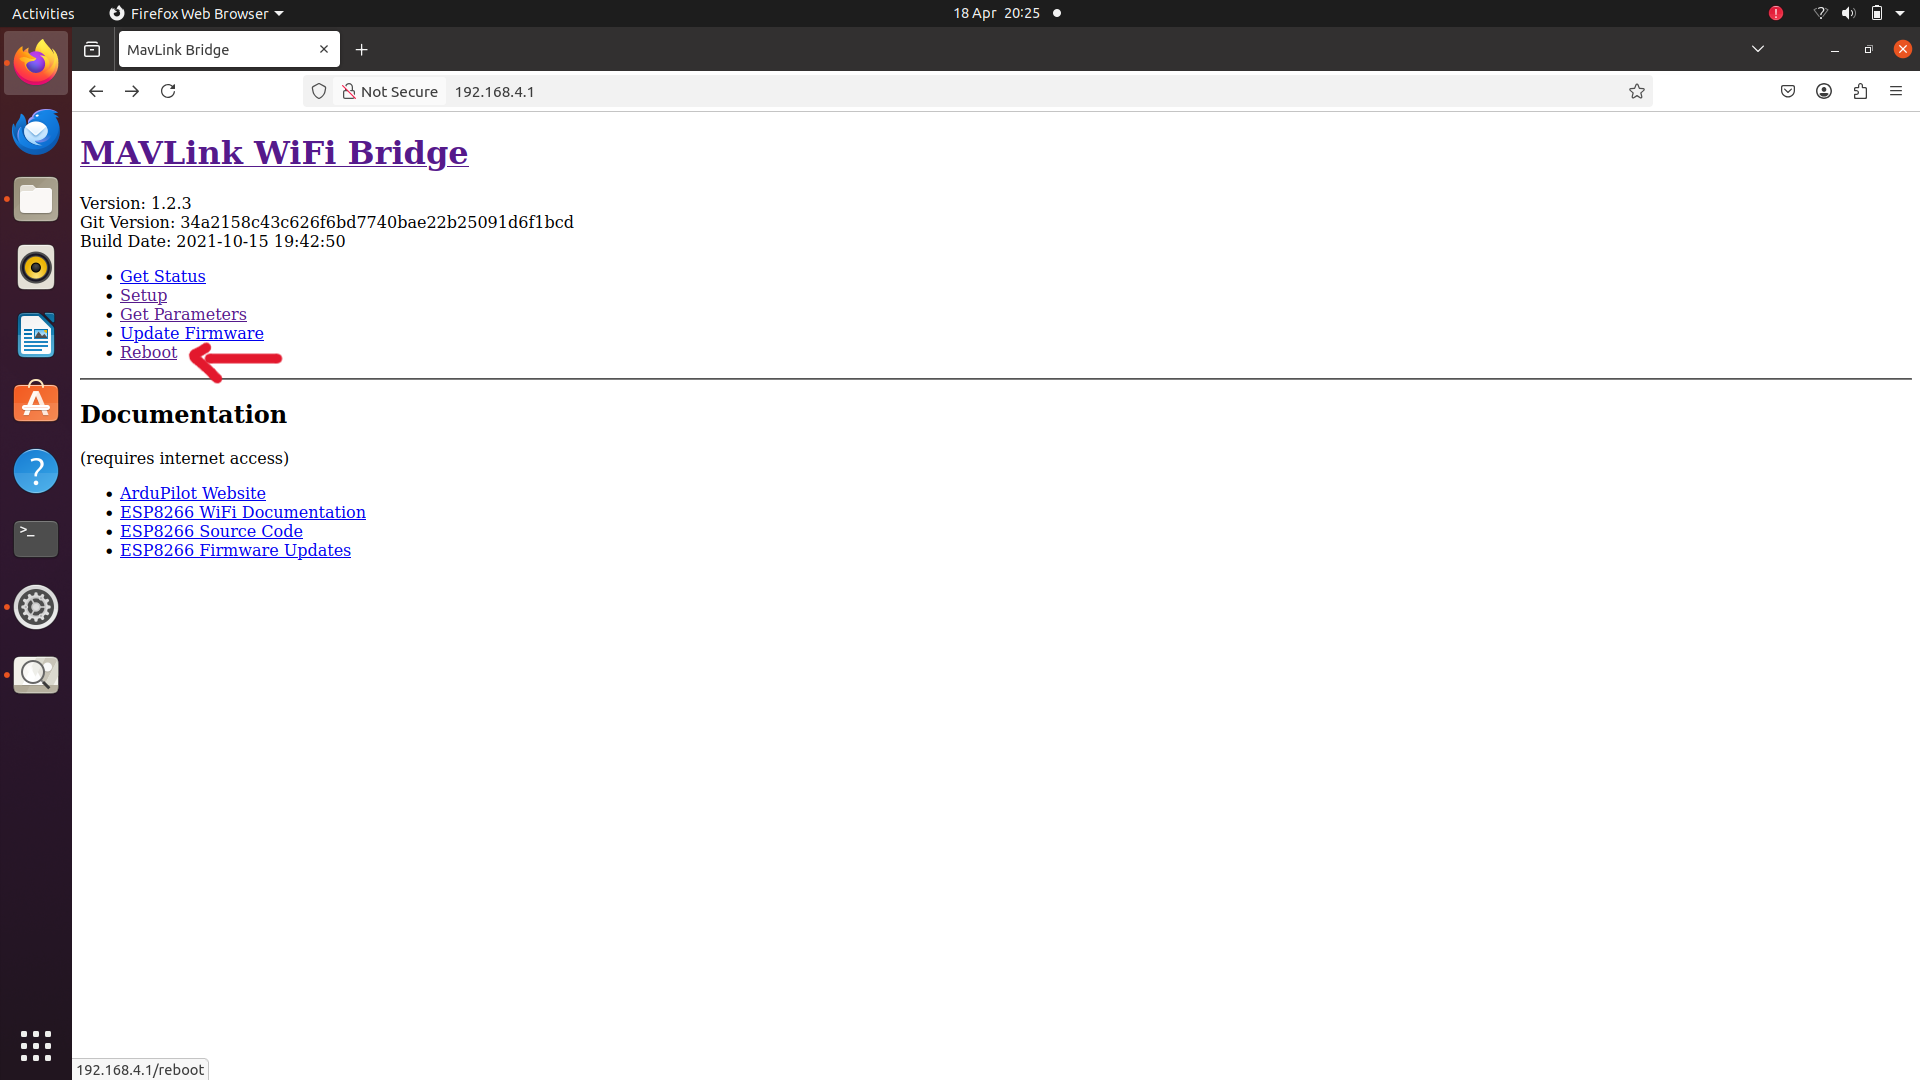
\includegraphics[width=1\linewidth]{Images/Wifi9.png}
    \caption{Pinout from Pixhawk 6c to ESP8266.}
    \label{fig:wifi9}
\end{figure}
You now have a link between the ESP module and your GCS. Next, you now need to configure the Pixhawk so that it is compatable with the wifi module.  

\subsection{MissionPlanner Configuration}
Connect the usb-c port of the Pixhawk6C to a copmuter as shown in figure \ref{fig:mission0} below:

\begin{figure}[H]
    \centering
    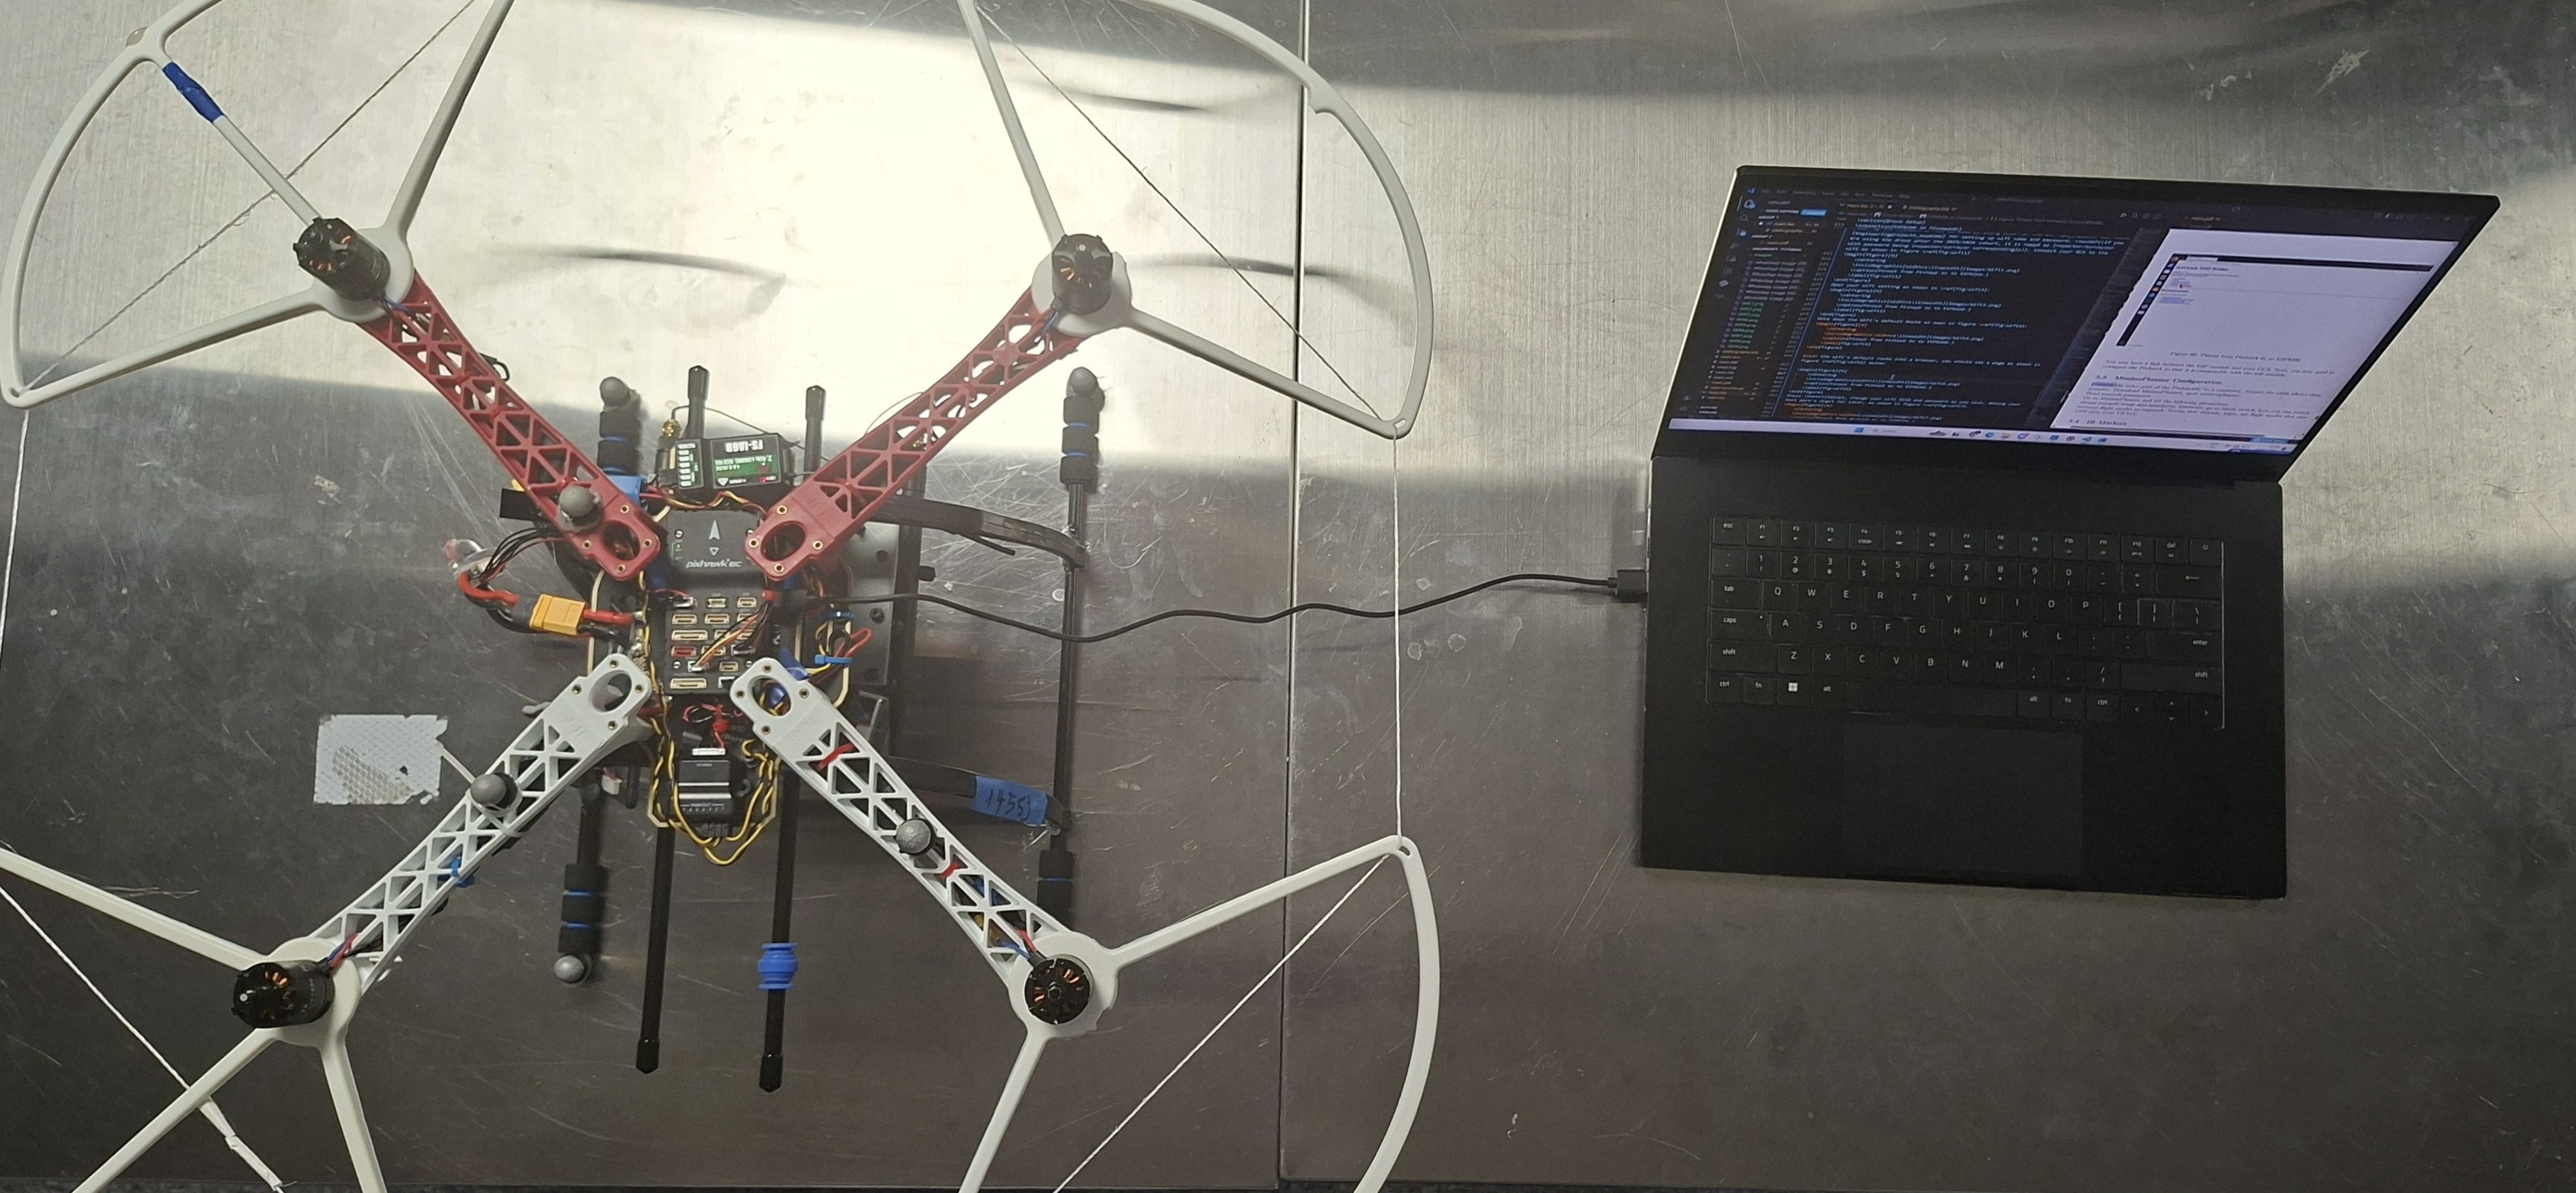
\includegraphics[width=1\linewidth]{Images/Mission0.jpg}
    \caption{Pinout from Pixhawk 6c to ESP8266.}
    \label{fig:mission0}
\end{figure}

Download MissionPlanner \cite{missionplanner_installation}. Open missionplanner and connect to the drone as seen in figure \ref{fig:mission1}:

\begin{figure}[H]
    \centering
    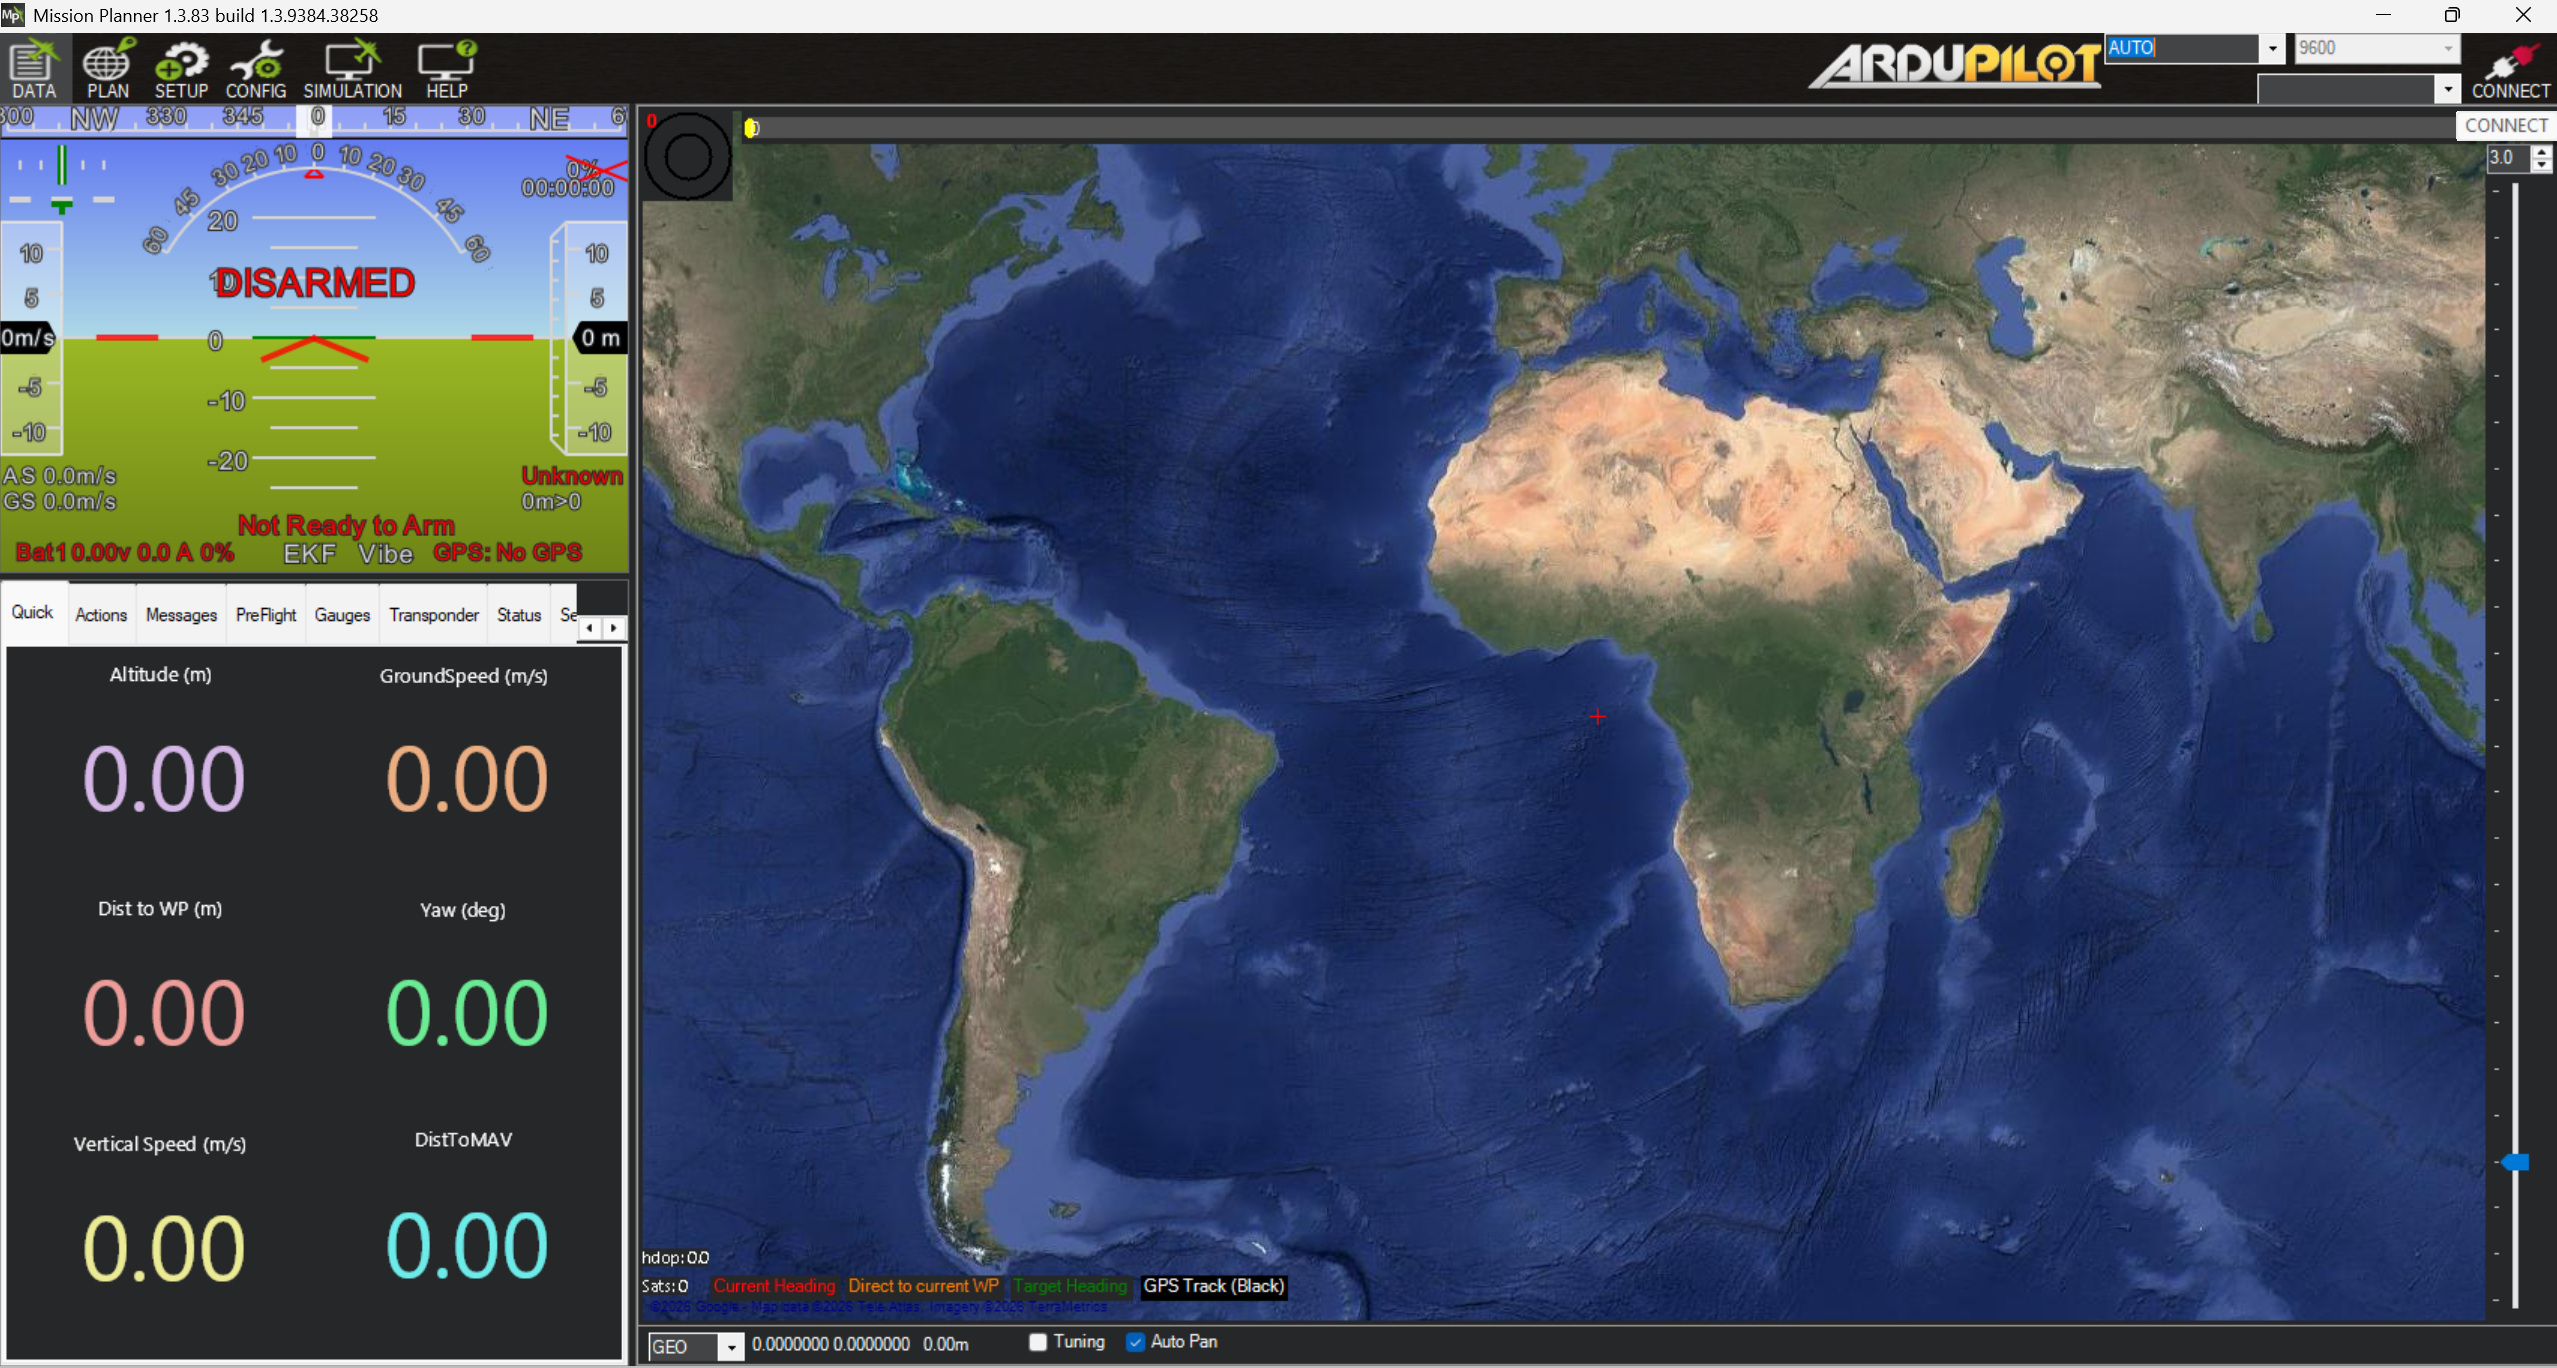
\includegraphics[width=1\linewidth]{Images/Mission1.png}
    \caption{Pinout from Pixhawk 6c to ESP8266.}
    \label{fig:mission1}
\end{figure}
On the top left, press \textit{Config}, then press \textit{Full Parameter List} shown on the left side panel, a warning will show up, press \textit{OK}, as seen below in figure \ref{fig:mission2}:
\begin{figure}[H]
    \centering
    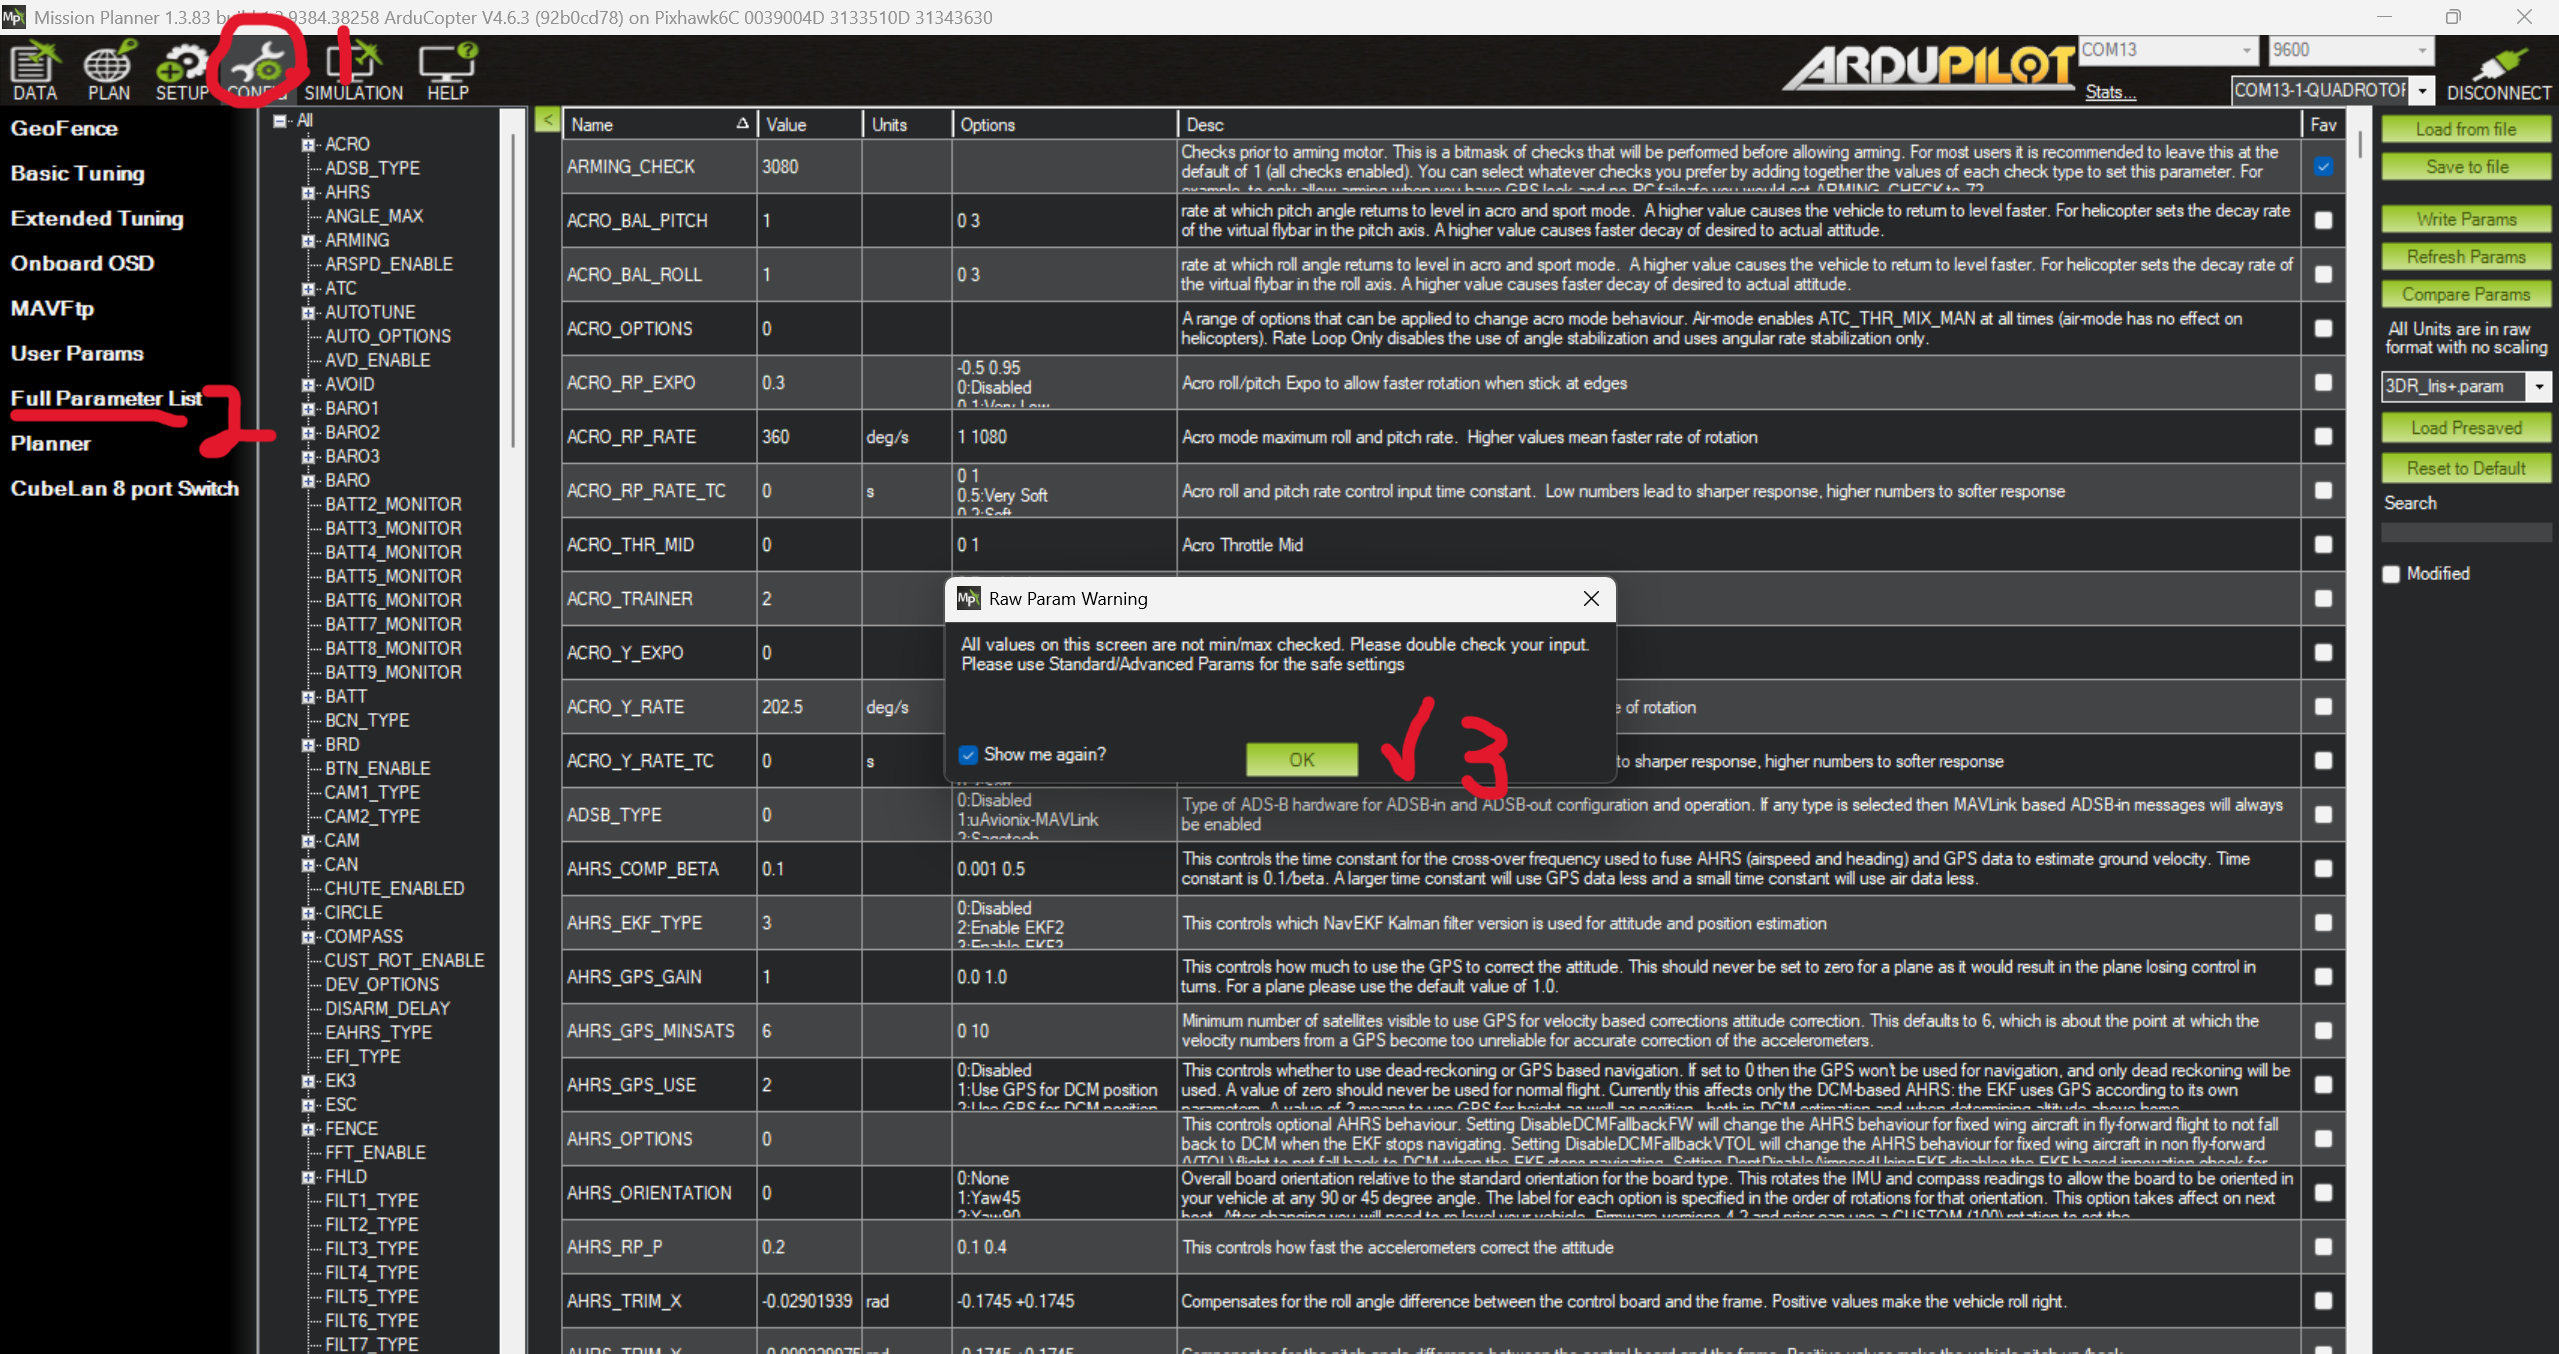
\includegraphics[width=1\linewidth]{Images/Mission2.png}
    \caption{Pinout from Pixhawk 6c to ESP8266.}
    \label{fig:mission2}
\end{figure}
Search for \textit{AHRS EKF TYPE 3} in the searchbox on the right panel, then change the value of it to \textit{3}, press \textit{Write Params} on the right panel, as seen below in figure \ref{fig:mission3}:
\begin{figure}[H]
    \centering
    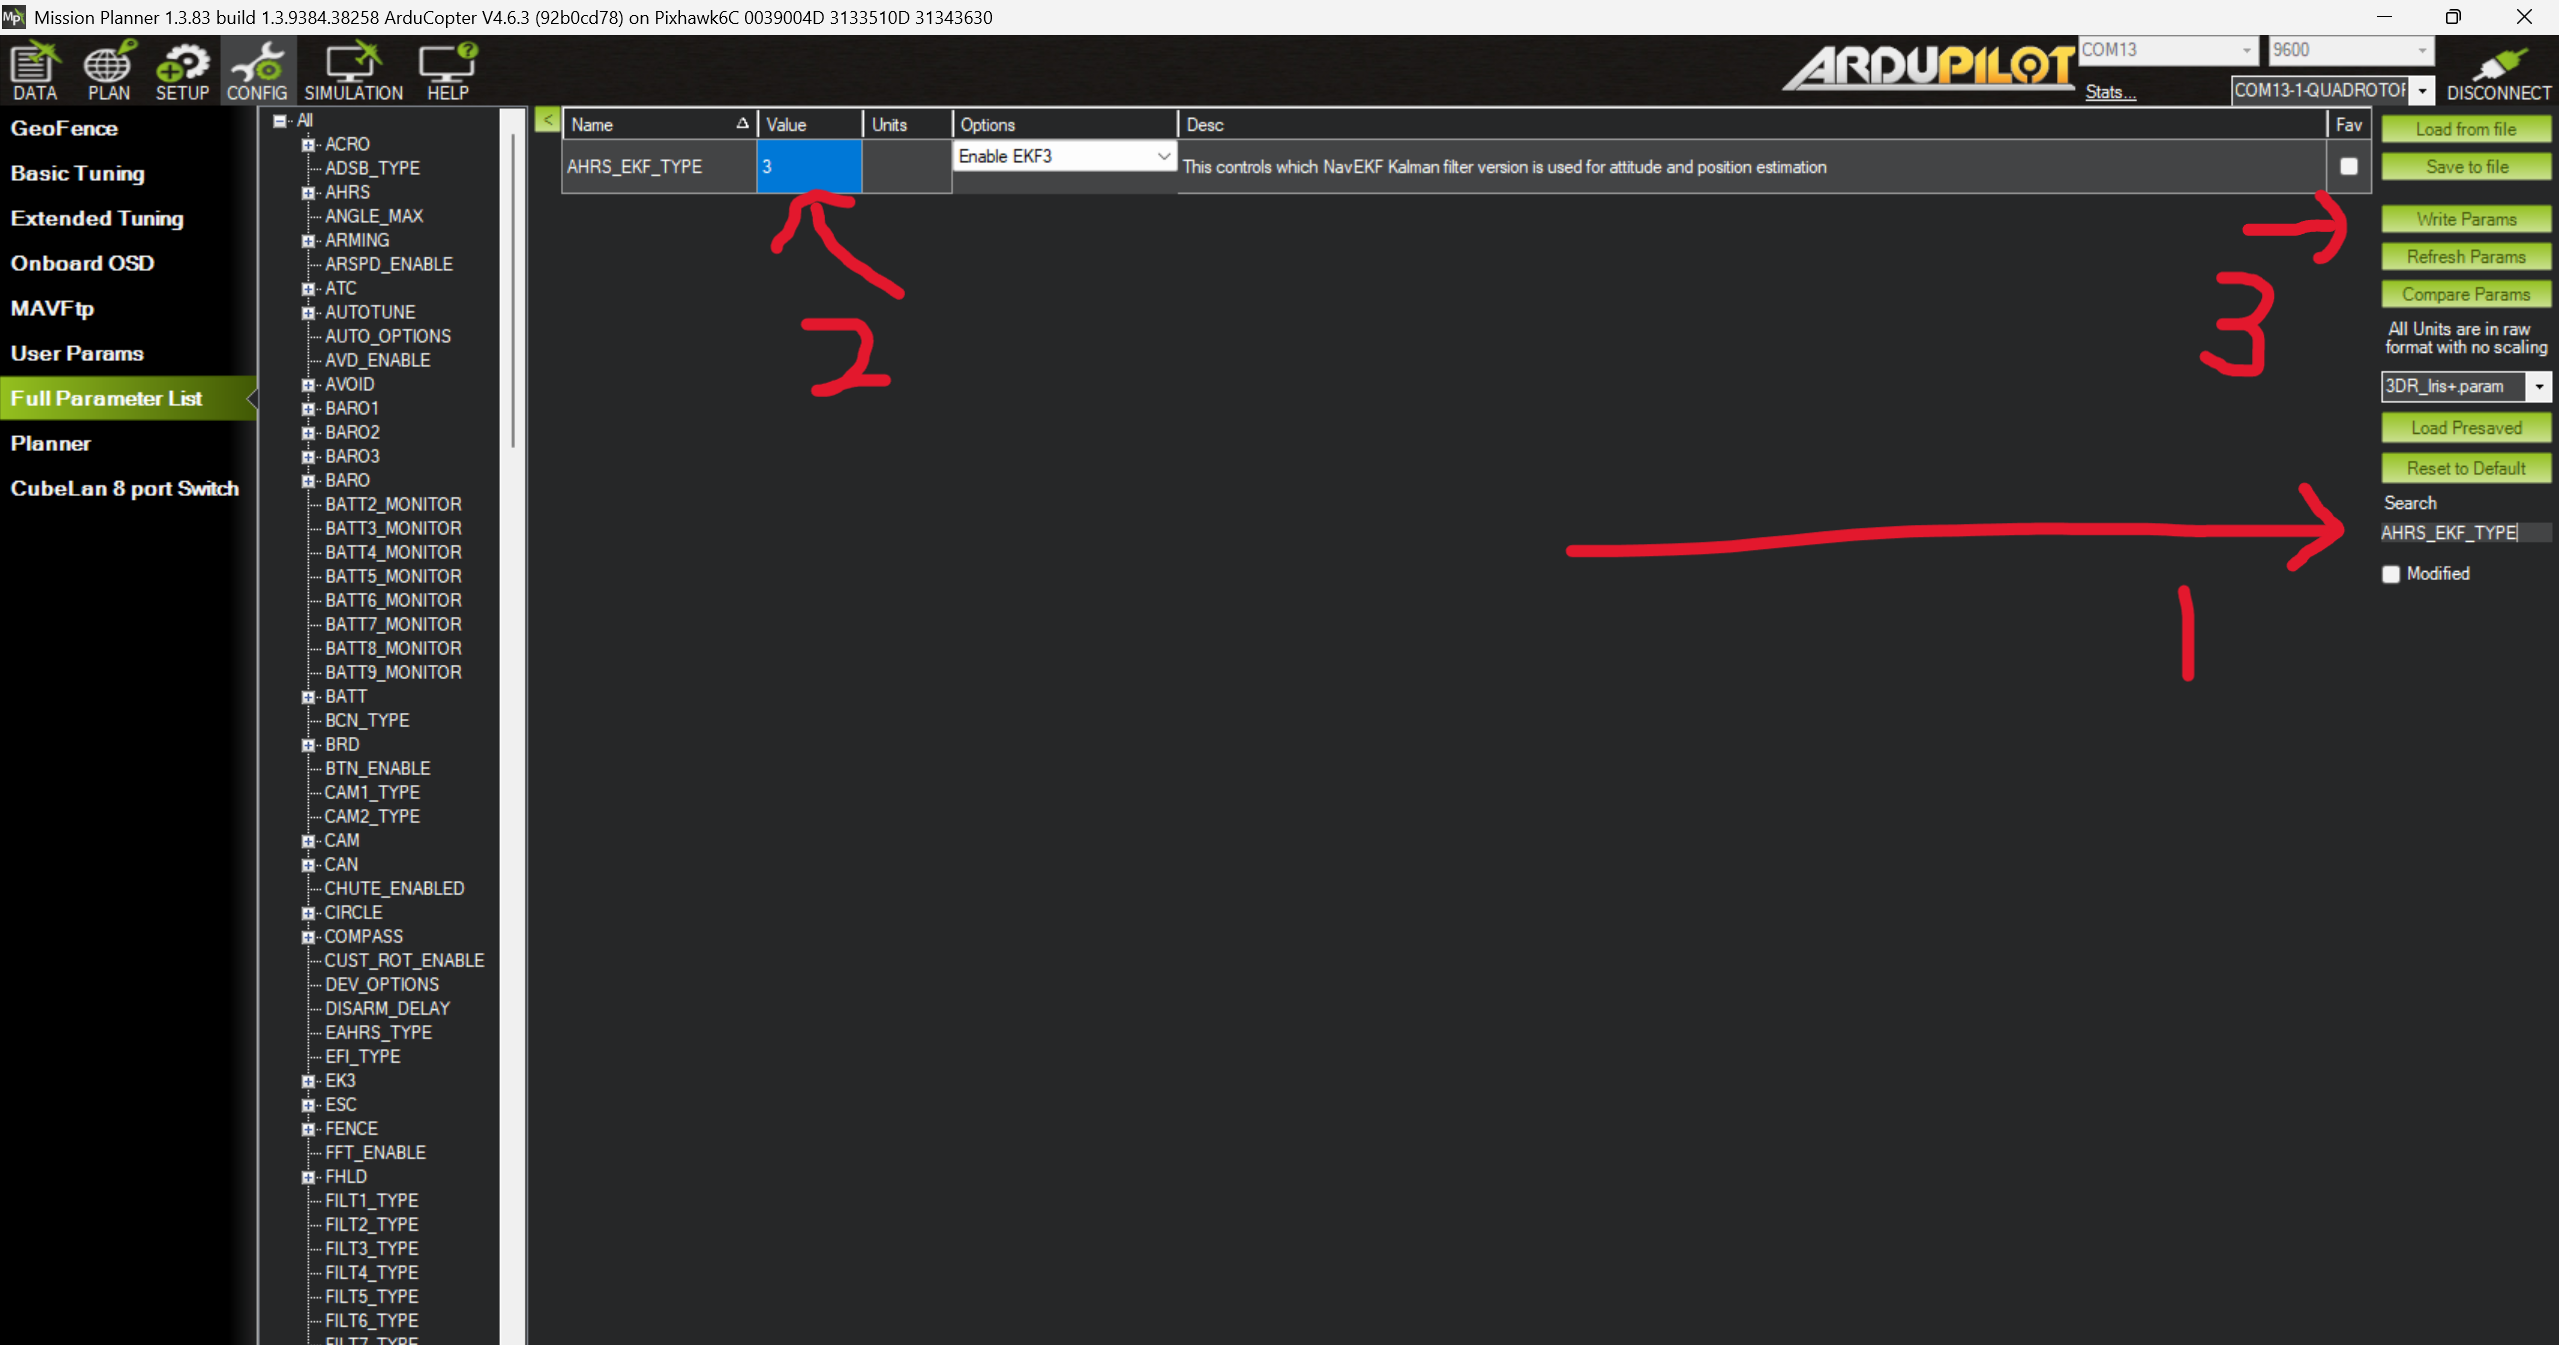
\includegraphics[width=1\linewidth]{Images/Mission3.png}
    \caption{Pinout from Pixhawk 6c to ESP8266.}
    \label{fig:mission3}
\end{figure}
A window will pop up asking for confrimation, click \textit{Yes} as shown in figure \ref{fig:mission4}
\begin{figure}[H]
    \centering
    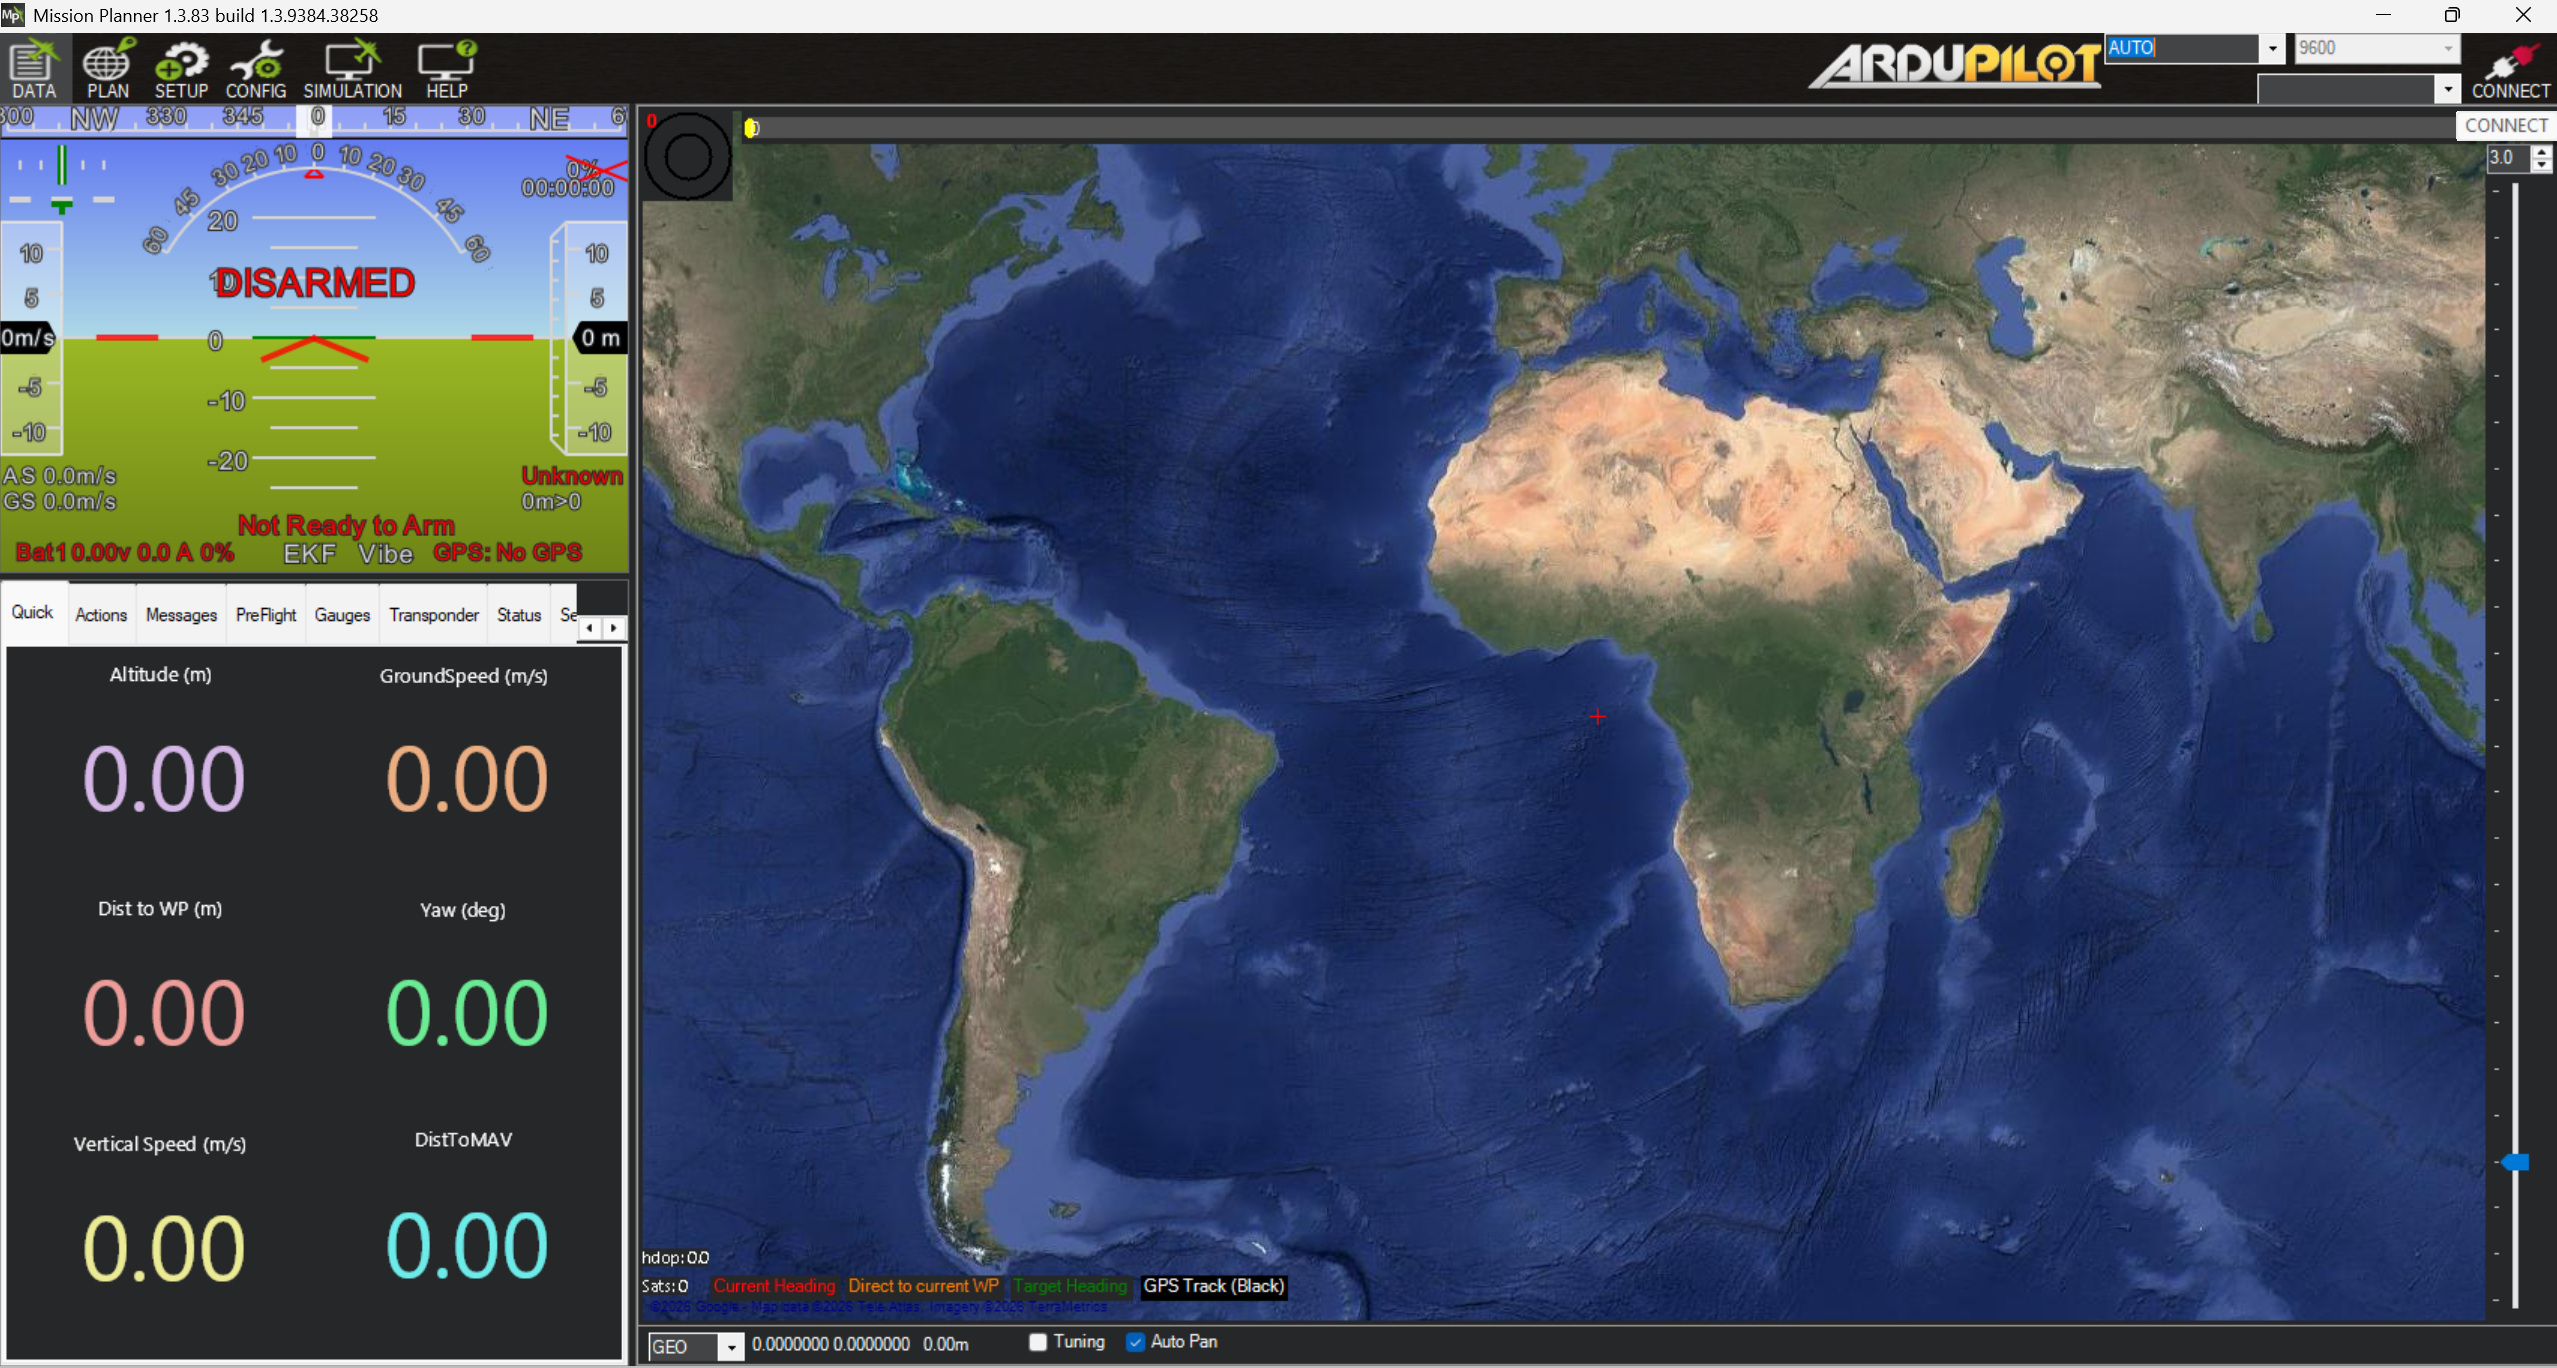
\includegraphics[width=1\linewidth]{Images/Mission1.png}
    \caption{Pinout from Pixhawk 6c to ESP8266.}
    \label{fig:mission4}
\end{figure}
Once confirmed, the value is now saved to the Pixhawk6c flight controller, a confirmation message will be shown like figure \ref{fig:mission5}.
\begin{figure}[H]
    \centering
    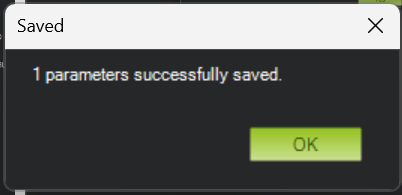
\includegraphics[width=0.5\linewidth]{Images/Mission5.png}
    \caption{Pinout from Pixhawk 6c to ESP8266.}
    \label{fig:mission5}
\end{figure}
Please also rewrite the all the variables shown in table \ref{tab:table}. 
\begin{table}[h!]
\centering
\caption{Configured ArduPilot Parameters}
\label{tab:table}   
\begin{tabular}{l l}
\hline
\textbf{Parameter} & \textbf{Value} \\
\hline
AHRS\_EKF\_TYPE & 3 \\
SERIAL1\_BAUD & 921 \\
SERIAL1\_OPTIONS & 2 \\
EK3\_SRC1\_POSXY & 3 \\
EK3\_SRC1\_POSZ & 3 \\
EK3\_SRC1\_VELXY & 3 \\
EK3\_SRC1\_VELZ & 3 \\
EK3\_SRC1\_YAW & 2 \\
EK3\_SRC2\_... & 0 \\
EK3\_SRC3\_... & 0 \\
EK3\_MAG\_CAL & 5 \\
EK3\_POSNE\_M\_NSE & 0.1 \\
GPS1\_TYPE & 14 \\
GPS1\_DELAY\_MS & 50 \\
COMPASS\_USE & 0 \\
COMPASS\_USE2 & 0 \\
COMPASS\_USE3 & 0 \\
\hline
\end{tabular}
\end{table}


Head towards \textit{SETUP}, \textit{Flight Modes}, you should navigate to a screen as shown in figure \ref{fig:mission6}.
\begin{figure}[H]
    \centering
    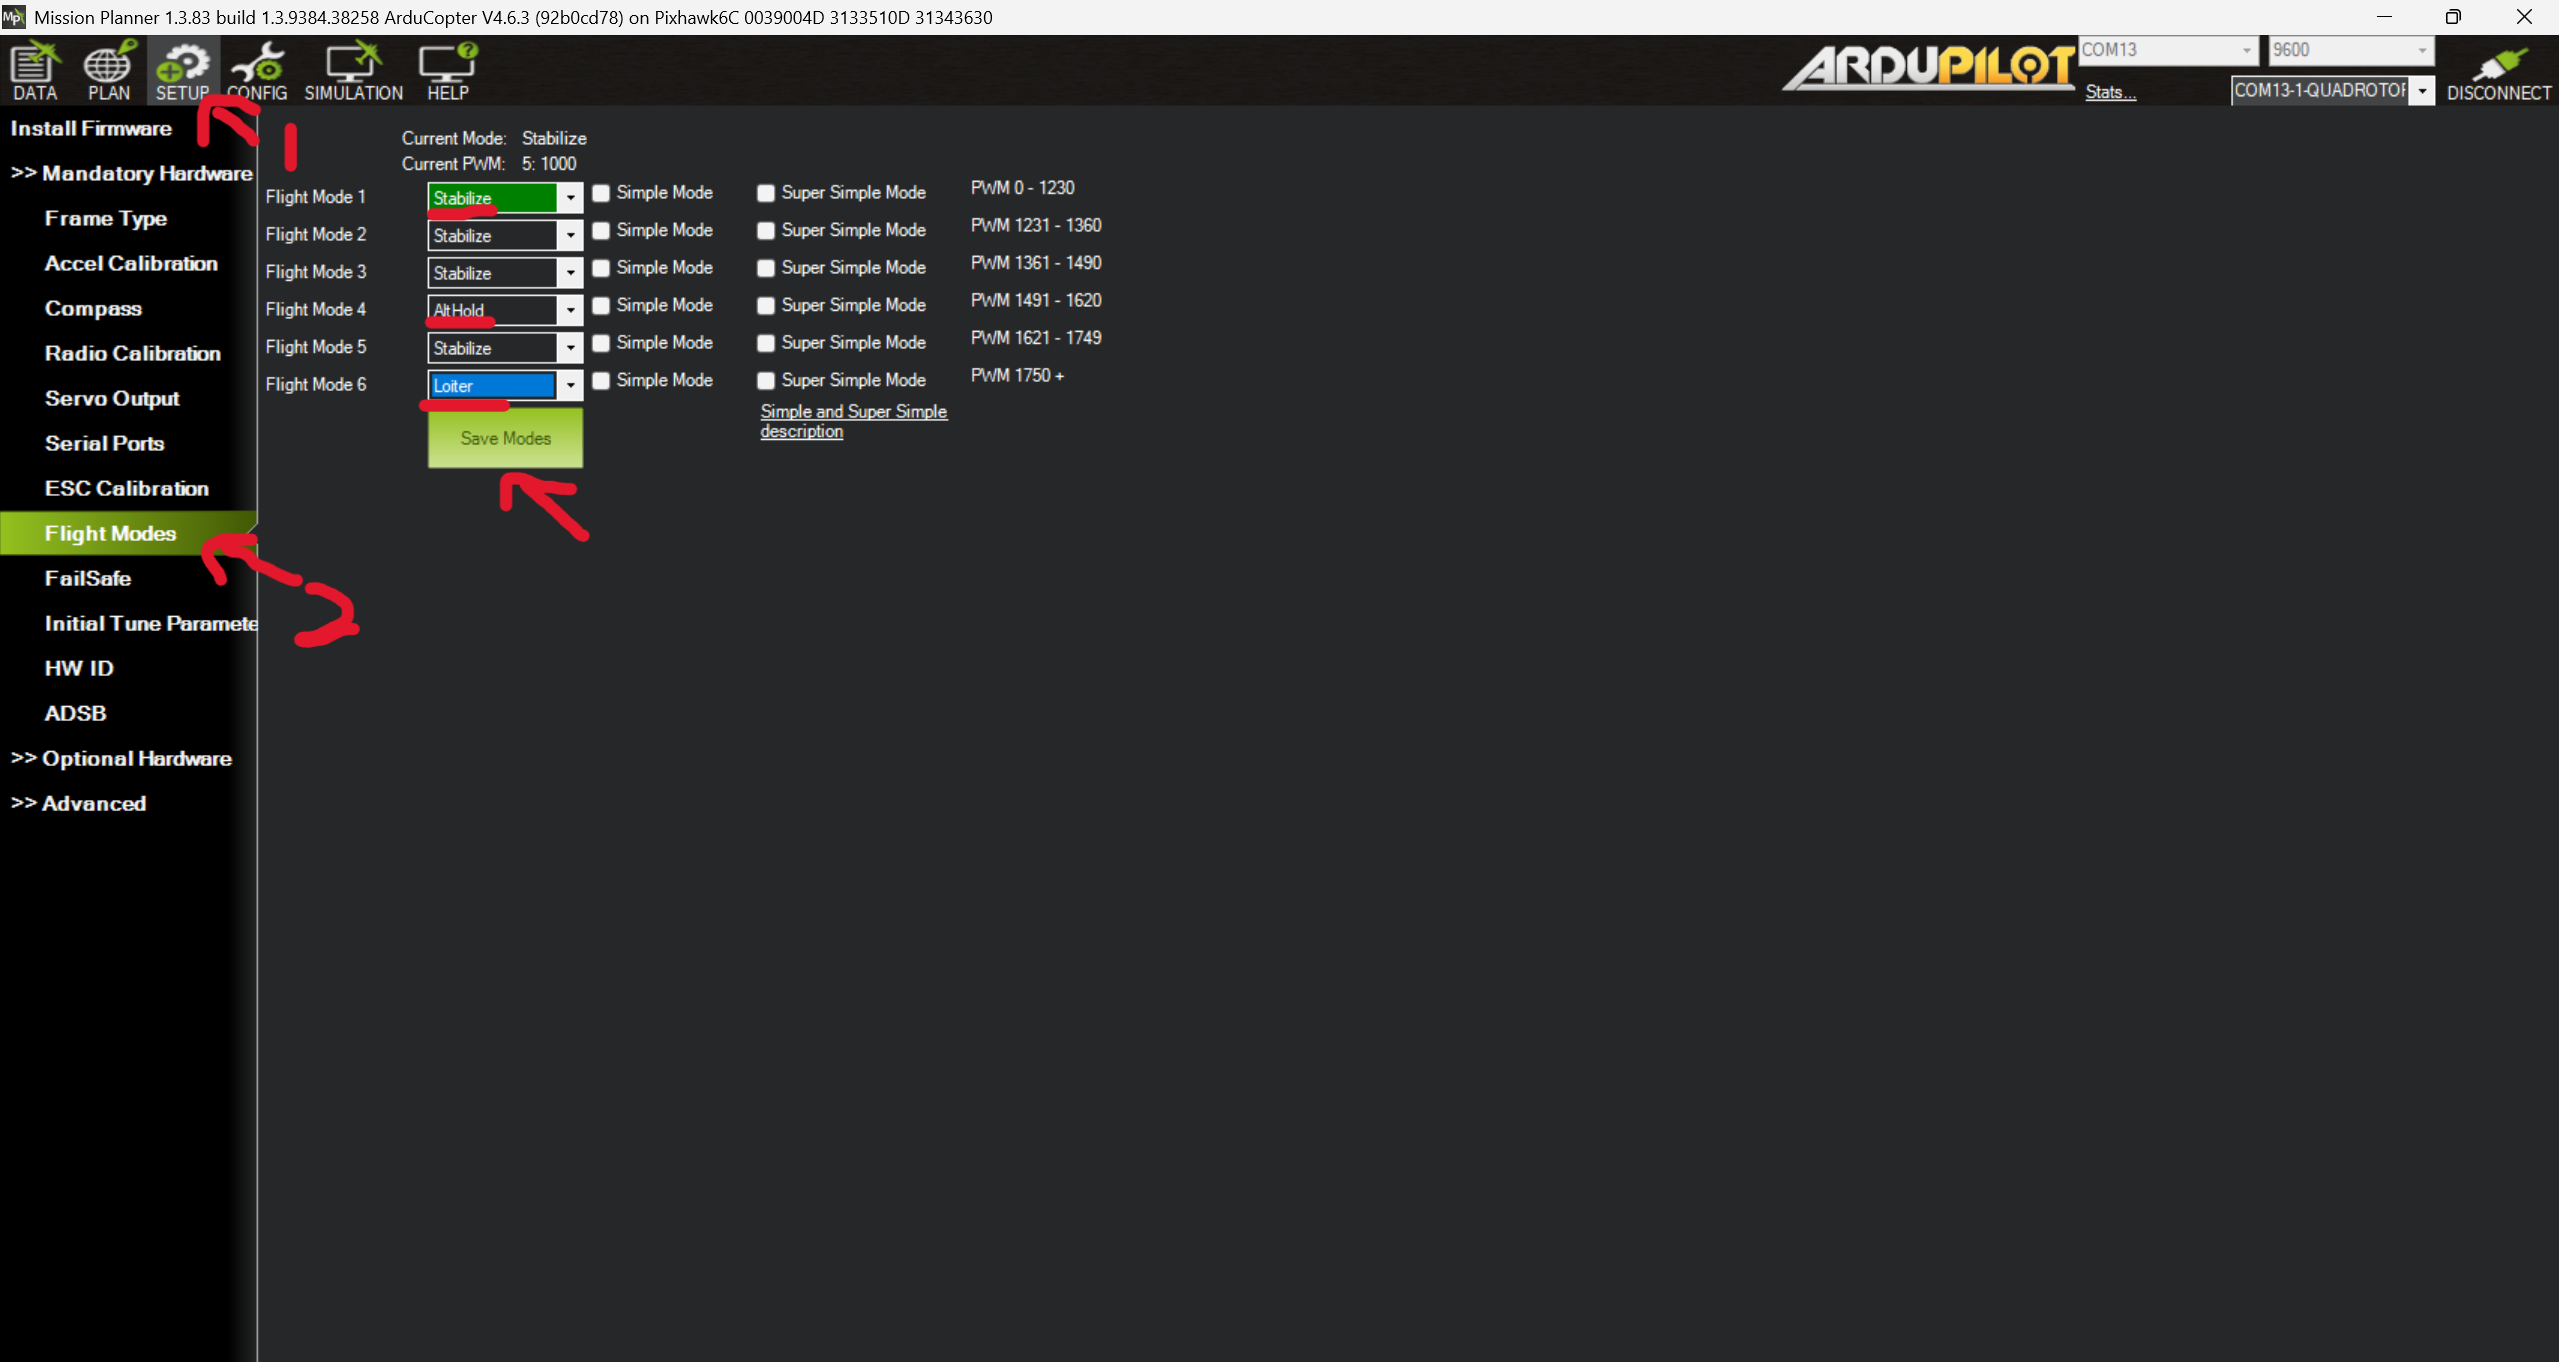
\includegraphics[width=1\linewidth]{Images/Mission6.png}
    \caption{Pinout from Pixhawk 6c to ESP8266.}
    \label{fig:mission6}
\end{figure}

Change the Flight Modes 1, 4, 6 into \textit{Stablize}, \textit{Alt Hold}, and \textit{Loiter}; Press \textit{Save Modes} to save your edits afterwards. Here I am using radio channel 5 on my transmitter, which corresponds to a 3 way switch, as my safety switch between Vicon indepedent flight mode to Vicon dependant flight mode,more information about the modes in section below.

\vspace{0.4cm} 

There is a general assumption here that you understand how to bind the transmitter to the recievers and how to map a switch into a flight mode. No worries if you don't know, there are plenty of Youtube tutorial that should cover this.


\subsection{Mavproxy Telemetry}
Now, Ardupilot is configured, return to the GCS and test if you recieve telemetry from your GCS!

Remeber to select the ESP8266 Wifi Network as shown in figure \ref{fig:GCST1}.


\begin{figure}[H]
    \centering
    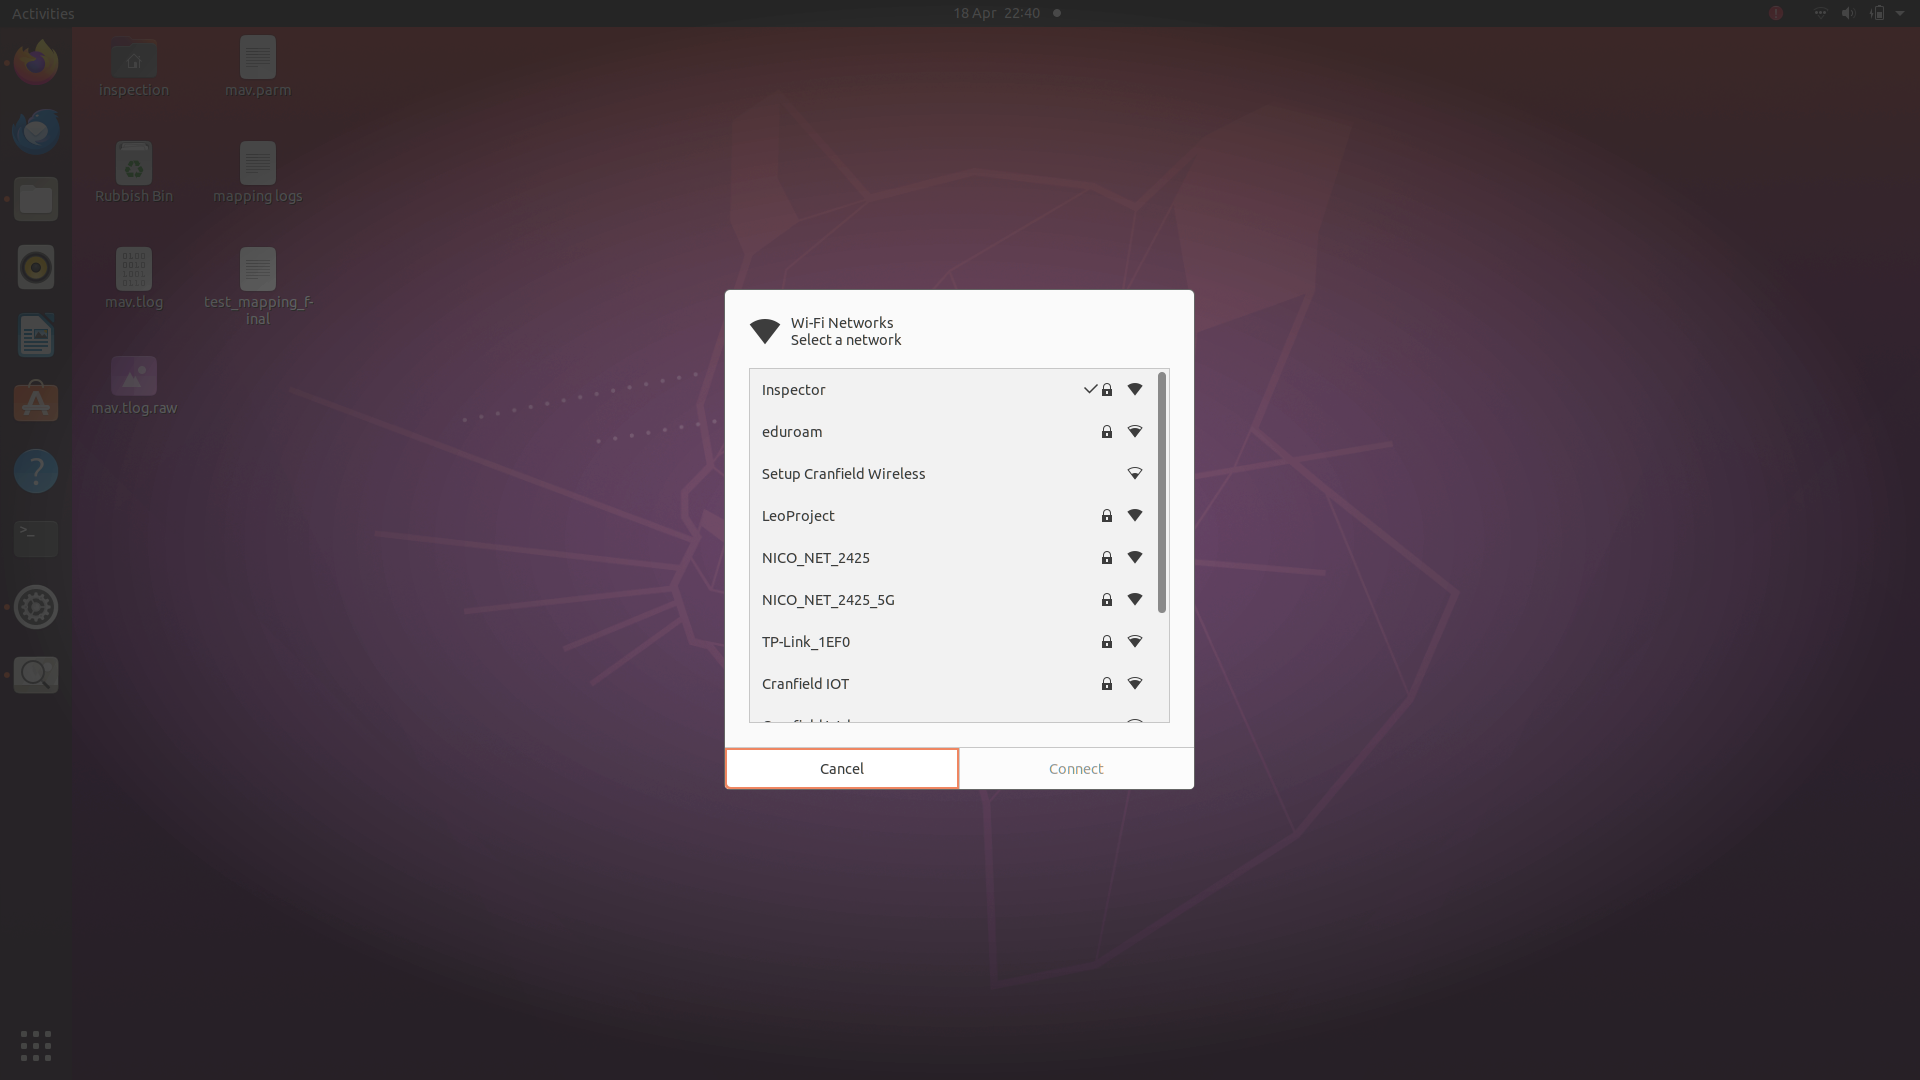
\includegraphics[width=1\linewidth]{Images/GCSTelem1.png}
    \caption{Pinout from Pixhawk 6c to ESP8266.}
    \label{fig:GCST1}
\end{figure}


Go to the GCS and type in the following: 

\begin{lstlisting}
    mavproxy.py --master :14554 --console --map
\end{lstlisting}

Recalling the Host Port number from section \ref{fig:wifi6}, replace 14554 with the number of your port. If successfully, telemetry should start showing up like figure \ref{fig:GCST3}, horray!
\begin{figure}[H]
    \centering
    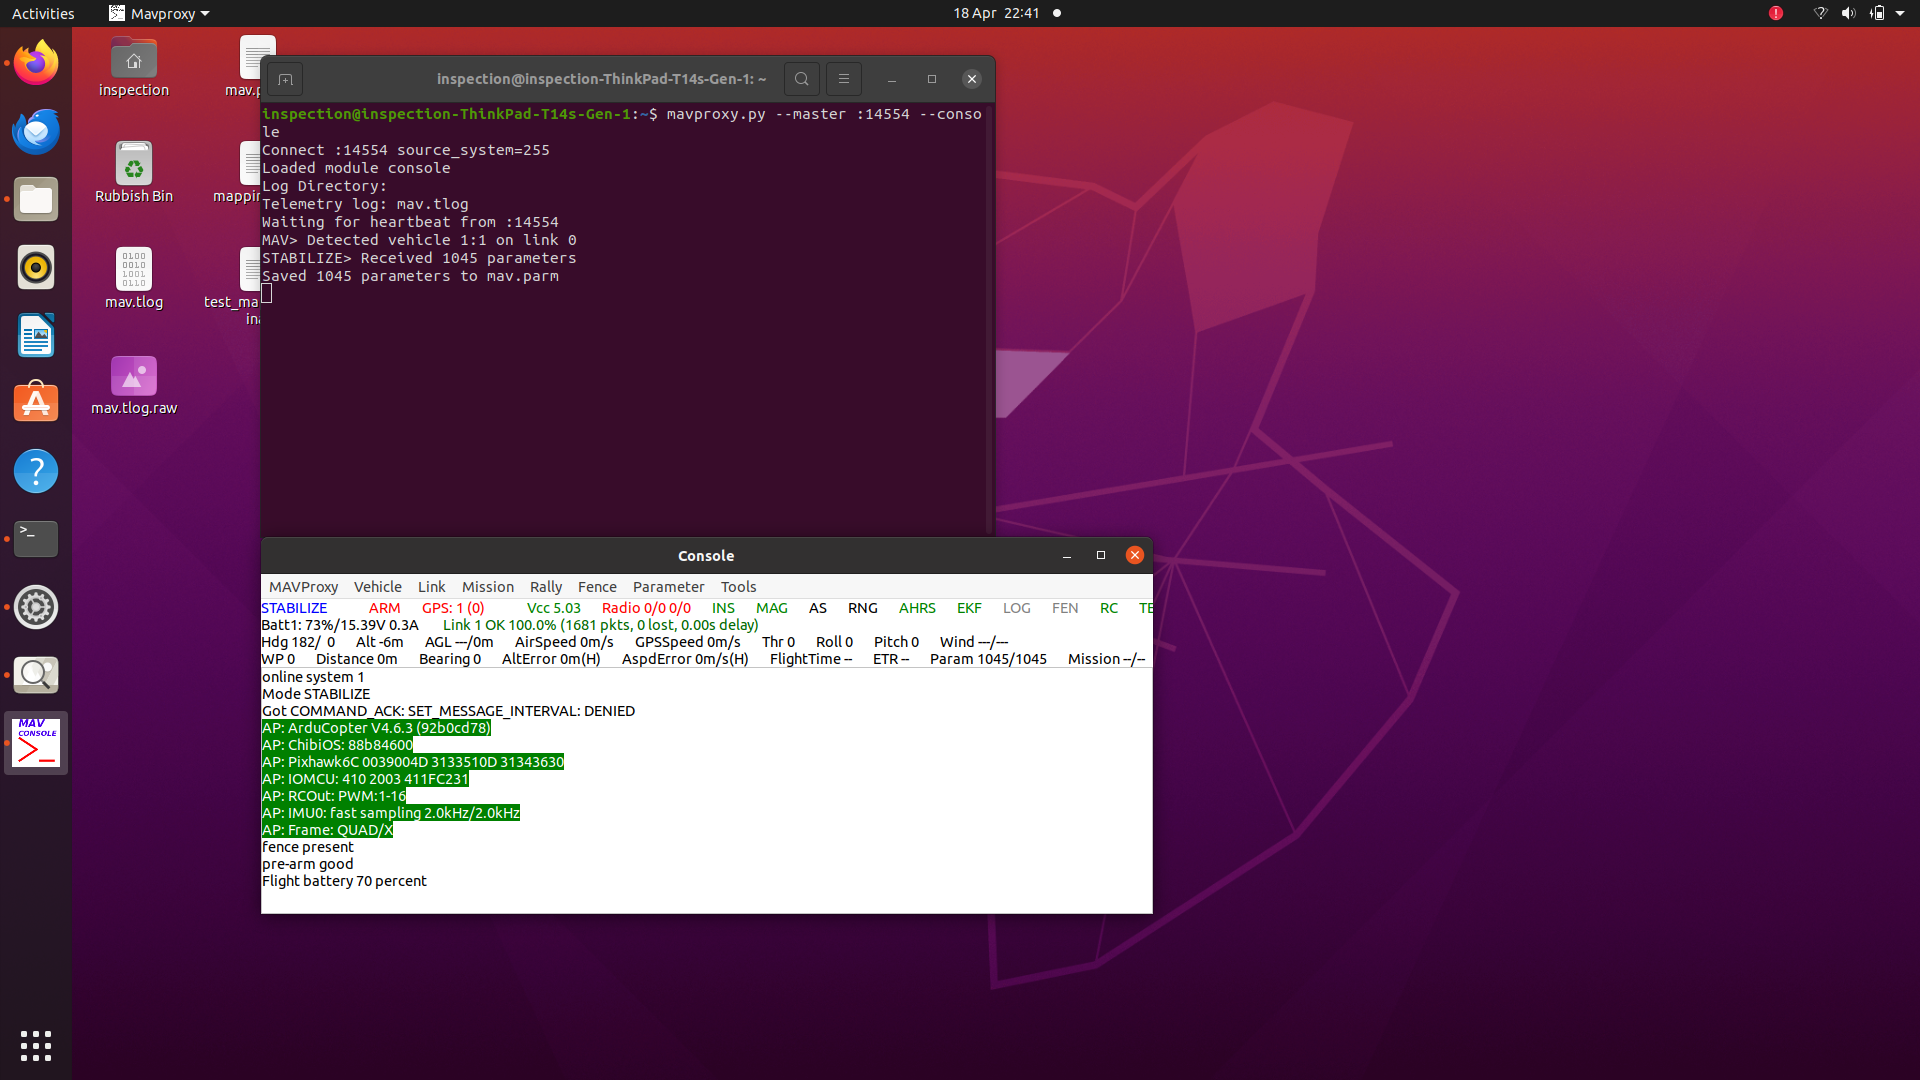
\includegraphics[width=1\linewidth]{Images/GCSTelem3.png}
    \caption{Pinout from Pixhawk 6c to ESP8266.}
    \label{fig:GCST3}
\end{figure}

\subsection{IR Markers}
Now your GCS connetions are all done, we are moving towards the final minors steps before actually flying the drone with VICON! Mount the IR markers with hot glue on location of your drones that is easily seen by the cameras. Have at least 4+ per drone and place them in an assymptical arragement, an example is shown in figure \ref{fig:irmarkers} below:  

\begin{figure}[H]
    \centering
    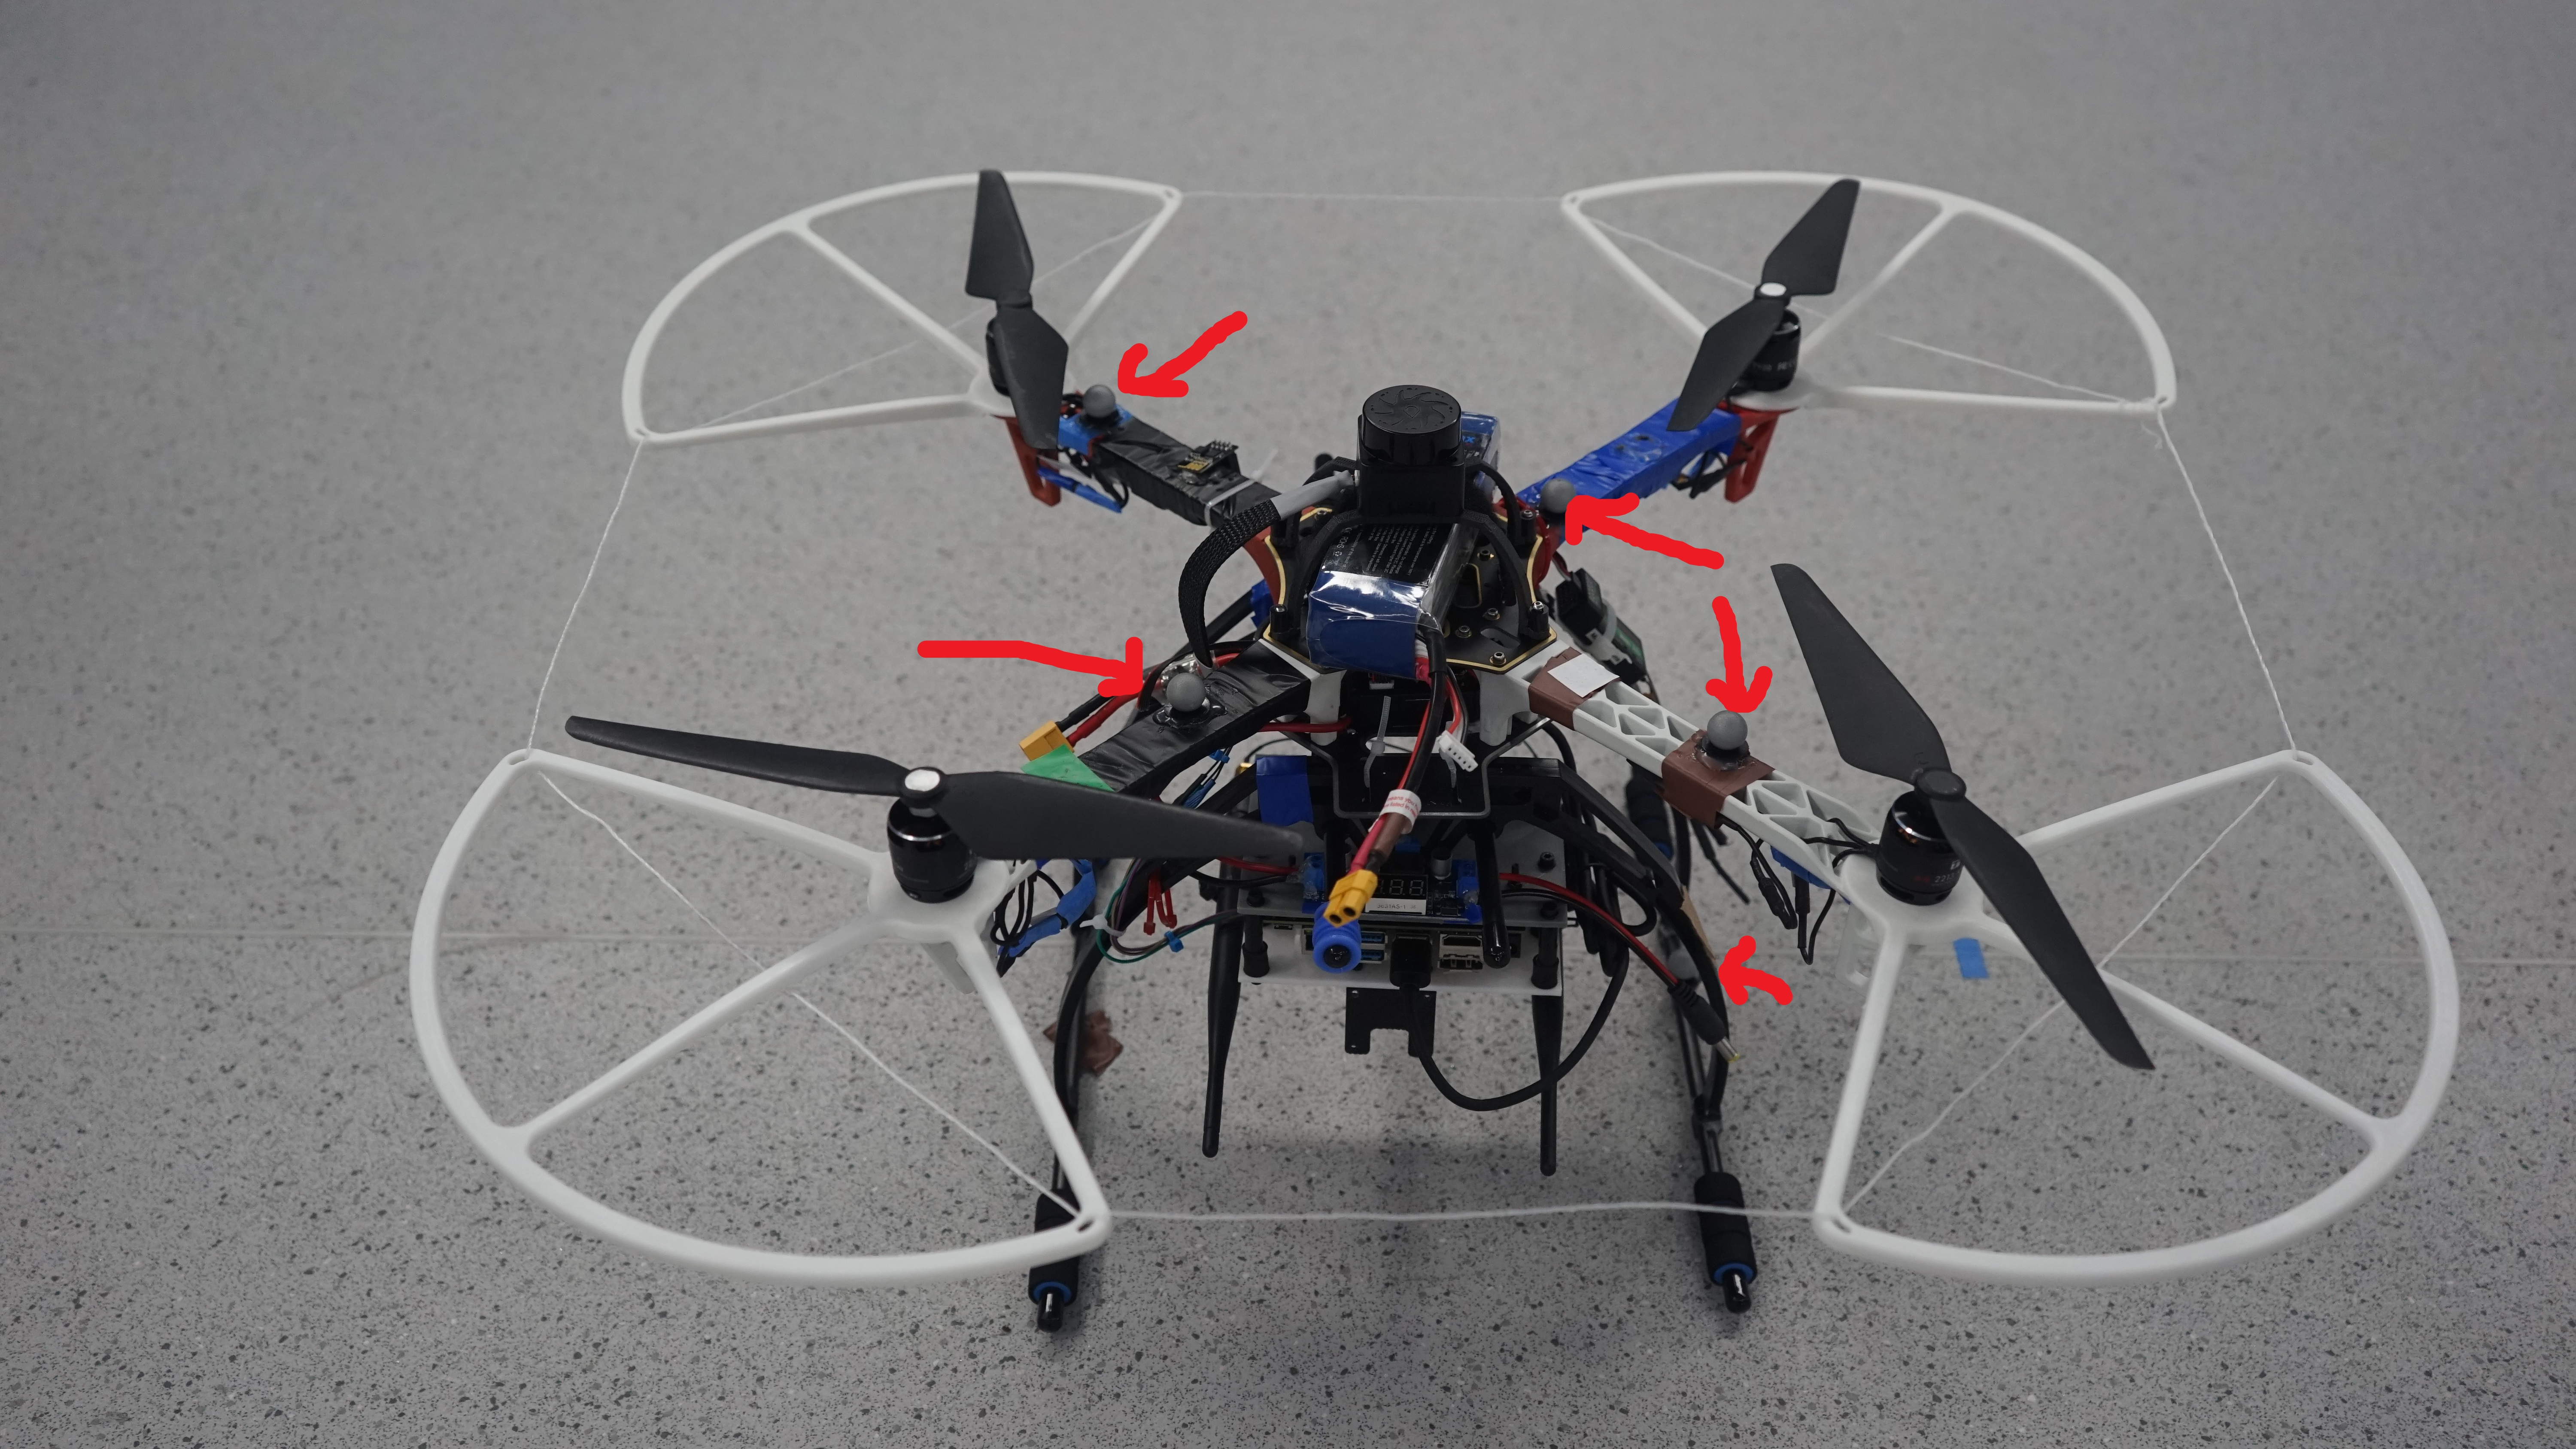
\includegraphics[width=1\linewidth]{Images/DSC05445.JPG}
    \caption{Example of Drone IR Markers layout.}
    \label{fig:irmarkers}
\end{figure}

If you are flying more than 1 drone, your assortment of IR markers must be geometrically different, otherwise the Vicon System may mistake the wrong object to track. (This has happened to me before and caused a crash.) 


\subsection{GCS to Vicon}
Finally, let's test the overall system. Plug in your GCS to the Vicon ethernet port as seen in figure \ref{fig:hardware}, connect the GCS laptop to the ESP8266's wifi, and place your drone inside the flight arena. \\
\vspace{0.4cm}
Setup the Vicon system by following section \ref{sec:viconsetup} above. This includes turning on the cameras, creating a mask, calibrating cameras, setting the origin, and define your now ready to go drone as a new object in section \ref{sec:defineNewObject}. \\

\vspace{0.5cm} 

One last thing, we must let pyvicon know the name of the object so it knows which object to track. To do this, go to GCS's \textit{Files} app, and navigate to \textit{/Home/.local/lib/python3.x/site-packages/MAVProxy/modules} and open the file named \textit{mavproxy\_vicon.py}, as shown in figure \ref{fig:NC1}:

\begin{figure}[H]
    \centering
    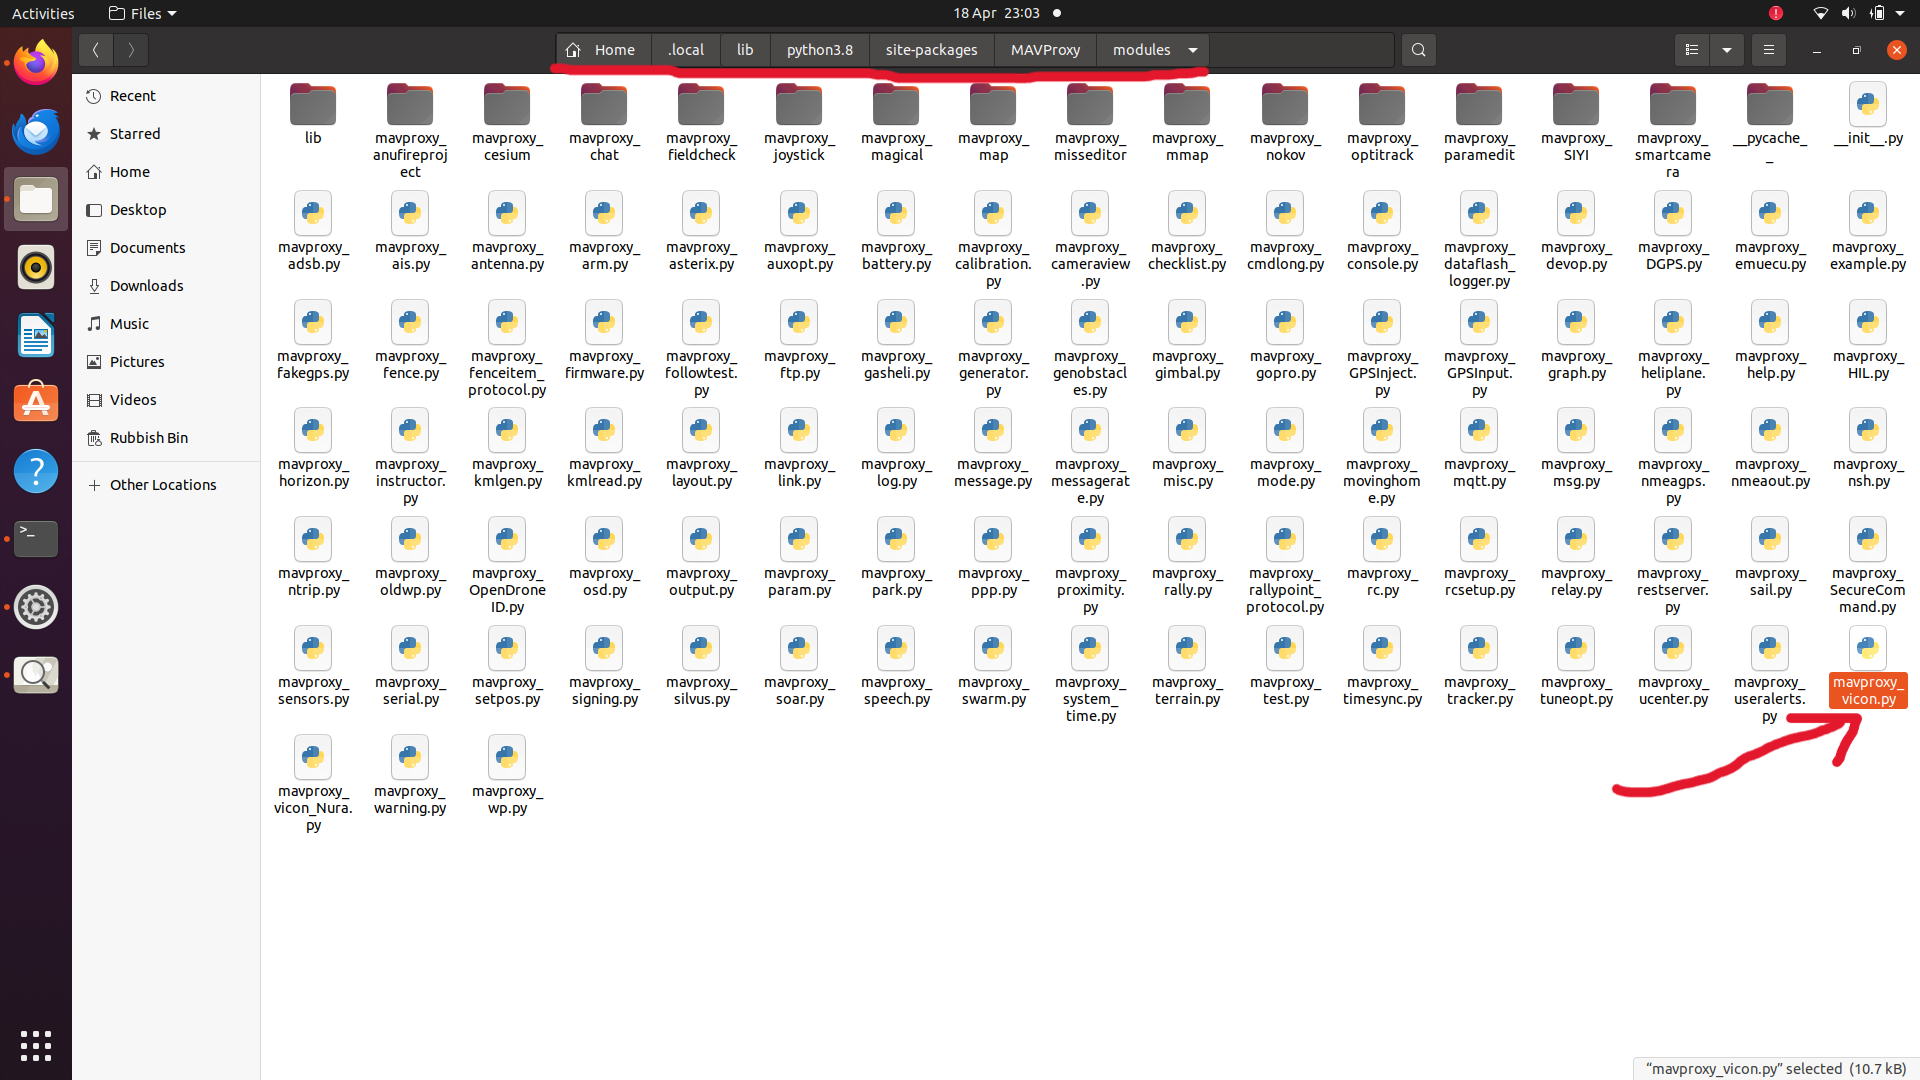
\includegraphics[width=1\linewidth]{Images/NameChange1.png}
    \caption{Example of Drone IR Markers layout.}
    \label{fig:NC1}
\end{figure}

If \textit{.local} can't be found on \textit{Home}, you can \textit{Show Hidden File} by pressing the button with 3 bars on top right. as shown in figure below:
\begin{figure}[H]
    \centering
    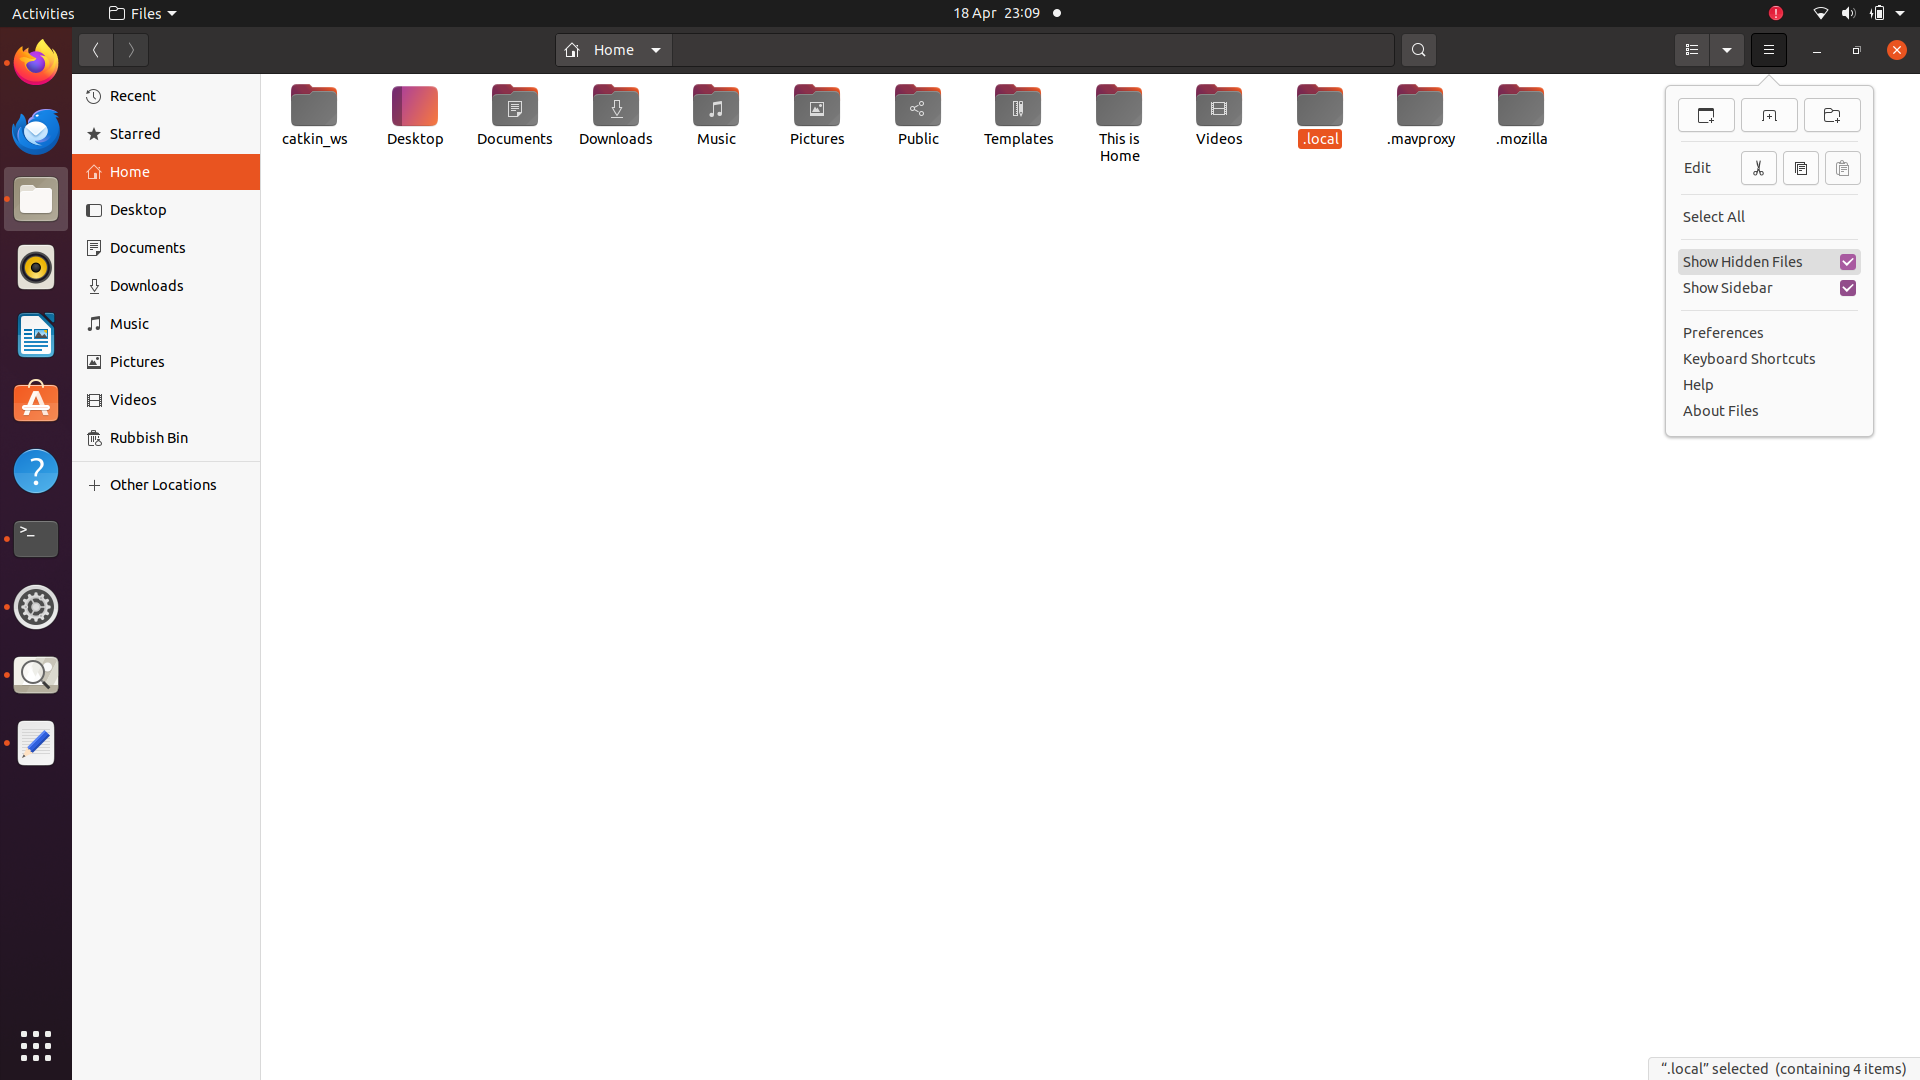
\includegraphics[width=1\linewidth]{Images/NameChange3.png}
    \caption{Example of Drone IR Markers layout.}
    \label{fig:irmarkers}
\end{figure}

Align your focus on line 29 to 36, and change \textit{(origin\_lat)(origin\_lon)(origin\_alt)} to 0. \textit{(object\_name)} as your object name. Here, \textit{MATT\_INSPECTOR} is the name of my drone as defined within the Vicon Host PC, and the origin lat lon and alt refers to the position of the Vicon Origin as (0,0,0). This comes important later on when conducting pathplanning, otherwise your drone might fly to Australia :). Make sure to save the changes from pressing \textit{Save} on top right as shown below in figure \ref{fig:NC2}. 

\begin{figure}[H]
    \centering
    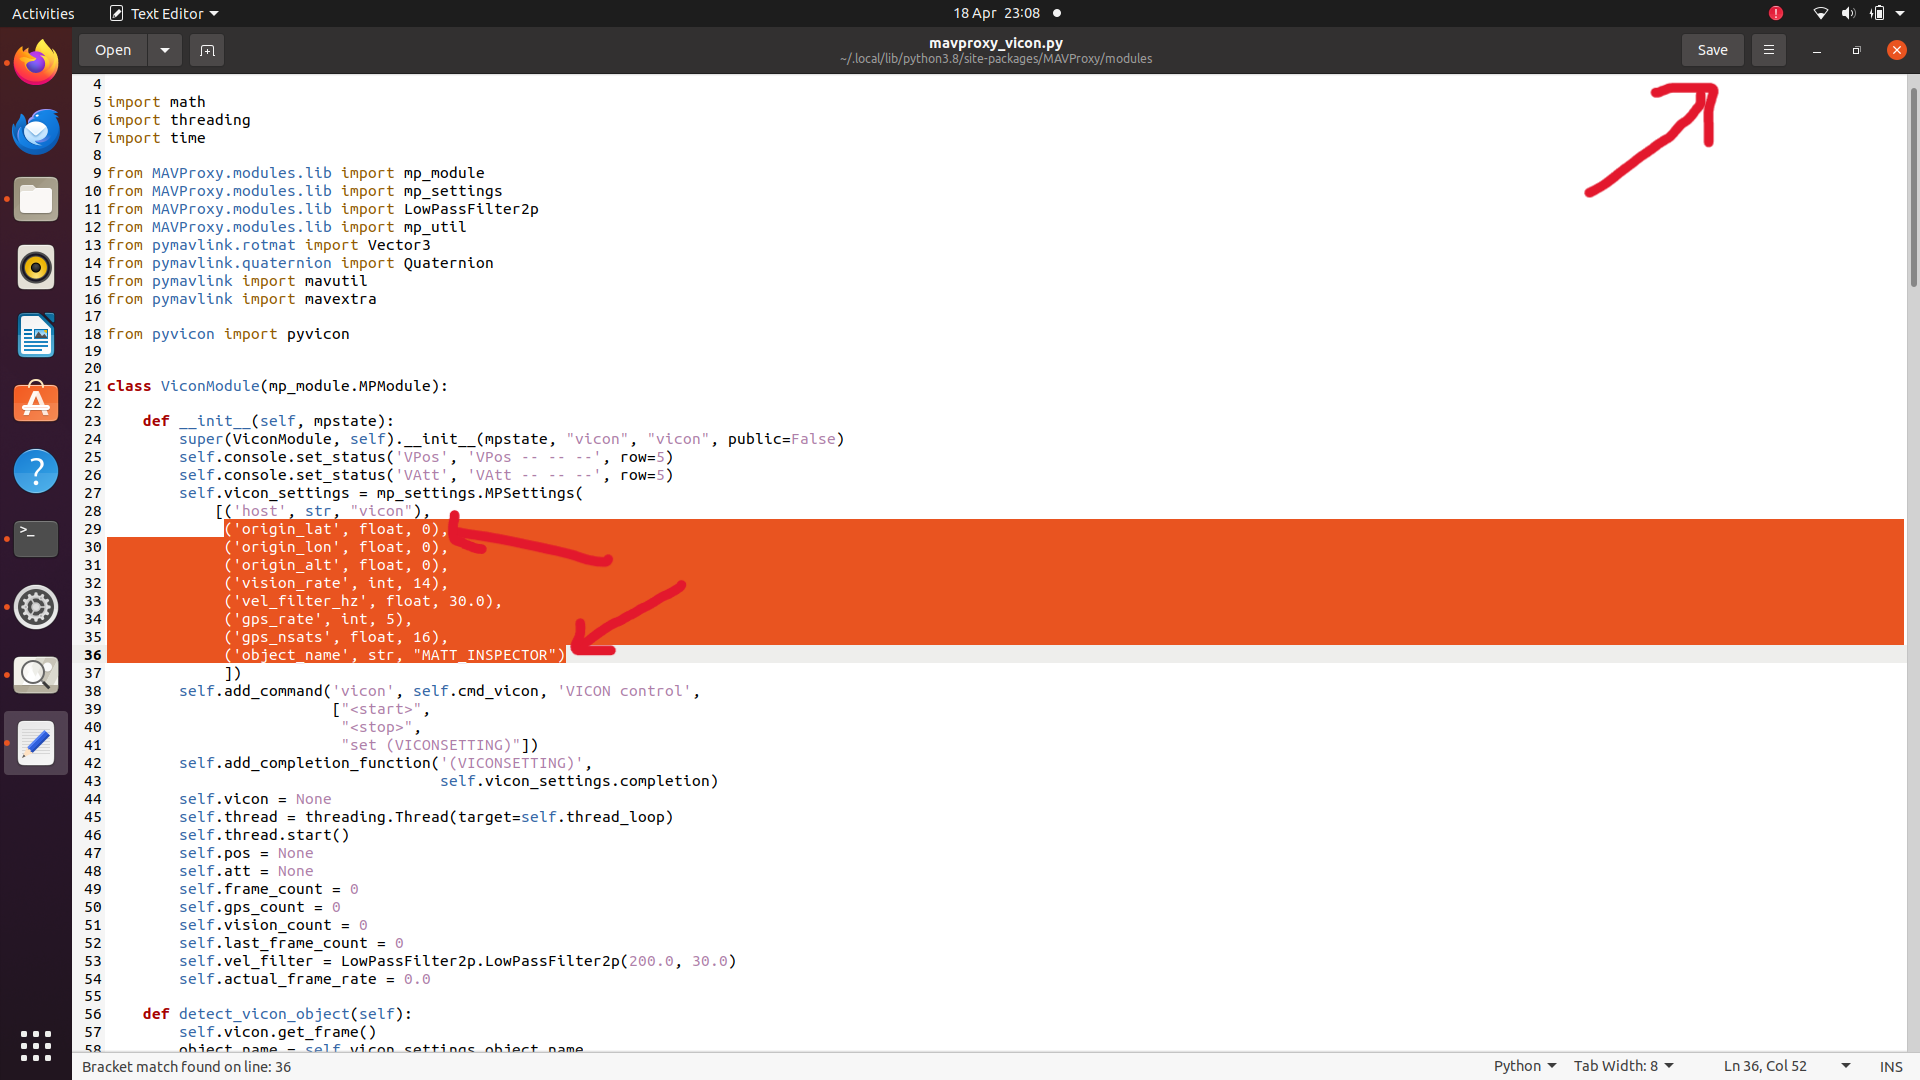
\includegraphics[width=1\linewidth]{Images/NameChange2.png}
    \caption{Example of Drone IR Markers layout.}
    \label{fig:NC2}
\end{figure}

Once completed, activate MAVproxy console, once again, this is done by opening terminal and typing:
 \begin{lstlisting}
    mavproxy.py --master :14554 --console --map
\end{lstlisting}

Within mavproxy, type the following to load the Vicon Module: 

 \begin{lstlisting}
    module load vicon
\end{lstlisting}

 \begin{lstlisting}
    vicon set
\end{lstlisting}

 \begin{lstlisting}
    vicon start
\end{lstlisting}

You should have the same results as figure \ref{fig:Works1}. A good way to verify if the object is being tracked correctly within the scirp is when entering \textit{vicon start}, it will only return the statement \textit{Connected to subject "MATT\_INSPECTOR" segment "MATT\_INSPECTOR} when it is working correctly.  

\begin{figure}[H]
    \centering
    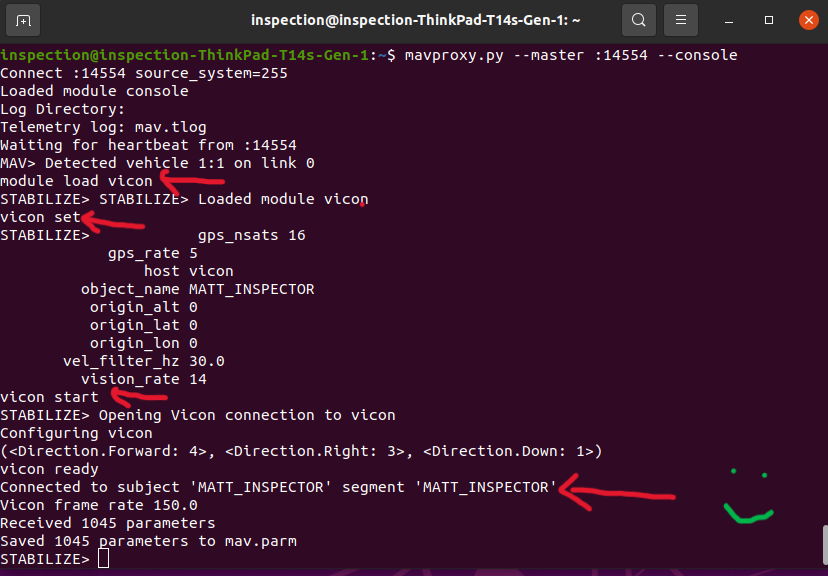
\includegraphics[width=0.9\linewidth]{Images/Works2.png}
    \caption{Example of Drone IR Markers layout.}
    \label{fig:Works1}
\end{figure}

If everything is working well, within the console, you should see the the NED (North East Down) and Euler angles (Roll Pitch Yaw) of your drone - Yippeee! \footnote{When console mentions height is at -12, this is referring a 12cm offset from the bottom to the center of the drone. As the position of the drone is defined as the geometric center of the assortment of IR markers you placed, this offset makes geometric sense.}
\begin{figure}[H]
    \centering
    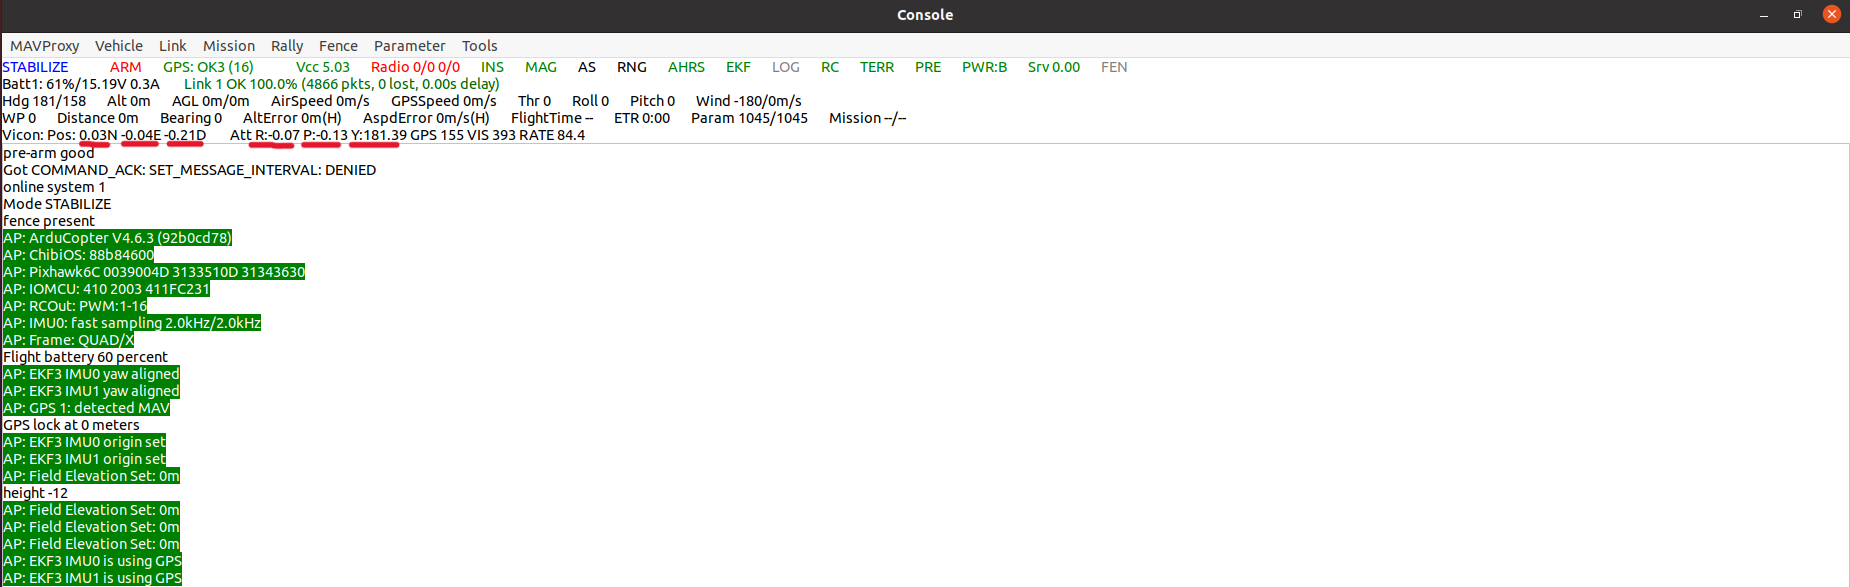
\includegraphics[width=1\linewidth]{Images/Works1.png}
    \caption{Example of Drone IR Markers layout.}
    \label{fig:NC2}
\end{figure}

\subsection{Finishing}
From this section, we have managed to merge the Vicon System, the GCS system you developed, and the drones that we prepared. We now have a working architecture that feeds Vicon postional data to the drone via the GCS. This is splendid and we are now ready for test flights!
\clearpage